\documentclass[11pt]{article}
\usepackage[utf8]{inputenc}
\usepackage[T1]{fontenc}
\usepackage[margin=1in]{geometry}
\usepackage{amsmath,amssymb,amsthm}
\usepackage{booktabs}
\usepackage{graphicx}
\usepackage{caption}
\usepackage{xcolor}
\usepackage[colorlinks=true,linkcolor=blue,citecolor=blue,urlcolor=blue]{hyperref}
\setlength{\emergencystretch}{3em}


\newtheorem{theorem}{Theorem}
\newtheorem{corollary}[theorem]{Corollary}
\newtheorem{proposition}[theorem]{Proposition}
\newtheorem{lemma}[theorem]{Lemma}
\newtheorem{conjecture}[theorem]{Conjecture}
\theoremstyle{remark}
\newtheorem*{remark}{Remark}
\graphicspath{{figures/}}

\title{\textbf{Keep the Angle}\\[2pt]
\large A Geometry-Preserving Basis in Spectral Embeddings}
\author{Andrew H. Bond\\
Department of Computer Engineering, San Jos\'e State University\\
\texttt{andrew.bond@sjsu.edu} ~\textbar~ ORCID: 0009-0003-2599-6158}
\date{Working draft --- v0.9}

\begin{document}
\maketitle

\begin{abstract}
The commute-time (resistance) embedding built from the low eigenvectors of a
graph Laplacian is a workhorse of spectral geometry, yet its distances degenerate
on large graphs (von~Luxburg, Radl, and Hein). We show the geometry does not
vanish: it is largely carried by the \emph{angular} coordinate. Writing each
node's low-mode embedding in polar form---magnitude times direction---the
direction preserves graph geodesics (Spearman $\rho\approx0.93$ on a reference
torus), while the magnitude, and an equal-size random-mode representation,
preserve almost none. Keeping only the direction is the row-normalization of
Ng--Jordan--Weiss spectral clustering applied to the commute-weighted embedding;
its existing theory (Schiebinger, Wainwright, and Yu) concerns cluster
separation, and we supply a metric-geometric account. An exact identity locates
the mechanism in \emph{tangential noncollapse}---the embedding velocity must not
turn purely radial---rather than in radius constancy; from it we prove a
deterministic angular-transfer theorem, a conditional graph-to-manifold result
(carried by the random-walk eigenvectors and the sup-norm eigenvector rates of
Calder, Garc\'ia Trillos, and Lewicka), and an \emph{unconditional} bi-Lipschitz
statement on an entire class of homogeneous spaces---flat tori, round spheres,
and every isotropy-irreducible homogeneous space---where Takahashi's
minimal-immersion theorem makes the normalized eigenmap an isometric immersion
into a sphere, closing both structural hypotheses and leaving only injectivity.
The radial claim is stated at three levels: proved
for the full embedding at intrinsic dimension $d\ge3$, empirical for the
truncated radius the algorithm computes, and borderline at $d=2$. Uniformity of
the metric constants in the mode count fails for the commute filter, but the
\emph{rank} form is uniform below dimension four: for $d\le3$ the angular ranking
converges to a fixed Green-kernel ranking, exact on the circle and on two-point
homogeneous spaces. The extended empirical program---substrate robustness across
graph families, a manifold diagnostic, and the fidelity--dimension trend---is the
companion Paper~I.b.
\end{abstract}

\noindent\textbf{Key words.} spectral embedding, commute-time (resistance) distance, row normalization, spectral clustering, geodesic distance, intrinsic dimension, Laplacian eigenmaps

\noindent\textbf{AMS subject classifications.} 05C50, 58J50, 62H30, 05C81, 68T09

\section{Introduction}
Spectral embeddings---Laplacian eigenmaps \cite{belkin2003}, diffusion and
commute-time maps \cite{coifman2006}---represent a graph by the low eigenvectors
of its Laplacian and underpin much of manifold learning and spectral clustering.
They carry a well-known pathology: on large geometric graphs the commute
(resistance) distance degenerates to a function of local degrees alone, losing
all global geometry \cite{vonluxburg2014}. Yet the most successful
spectral-clustering algorithm \cite{ng2002} \emph{row-normalizes} the
embedding---projects each node to the unit sphere---and works well. The
existing theory of that normalization concerns cluster geometry: it explains
why row-normalized embeddings of well-separated clusters concentrate in nearly
orthogonal directions on the sphere \cite{schiebinger2015,vonluxburg2008}. It
does not address metric geometry. Closer to our object, unit-hypersphere
normalization has been applied \emph{directly} to the commute-time embedding for
$3$D shape registration across differing samplings \cite{sharma2012}; there it is
a sampling-robustness heuristic, and the geodesic content of the resulting
angular distances is not analyzed. \textbf{This paper asks what row-normalization
recovers of the graph's geodesic structure, and why.}

Our answer is a clean decomposition. Write each node's low-mode embedding in polar
form, magnitude $\times$ direction. The \emph{magnitude} is the truncated,
normalized counterpart of the radial coordinate that von~Luxburg's theorem kills
for the \emph{full, unnormalized} commute embedding at $d\ge3$
(Corollary~\ref{thm:radial}); empirically it tracks local degree
(\S\ref{sec:verify}). The \emph{direction} carries
the graph's geodesic geometry (after the $\alpha{=}1$ density normalization
where sampling is strongly non-uniform, Paper~I.b). Row-normalization
keeps the direction and discards
the magnitude---so beyond its cluster-separation role it is also the
geodesically correct projection, and its fidelity is flat in both mode-count and
graph size precisely where the raw embedding decays.

The underlying operation---\emph{separate scale from direction, then keep the
part that carries the task geometry}---recurs beyond clustering: polar-coordinate
KV-cache quantization splits key vectors the same way \cite{polarquant2025},
evidence for the \emph{decomposition}, not for always discarding the radius. Our
hypotheses fix the boundary: discarding the magnitude is the right quotient
precisely when the radial variable is nuisance for the metric preserved---the
tangential-noncollapse condition (A2) of Theorem~\ref{thm:transfer}---which for
graph geodesics holds, the radius being degree/density noise
(Corollary~\ref{thm:radial}). On the reference torus the direction recovers
geodesics where the magnitude and a random-mode representation do not
(\S\ref{sec:results}); the companion Paper~I.b~\cite{paperIb} establishes the
basis's substrate-robustness and its failure modes across graph families.

\textbf{Contributions.} The first is the \textbf{Keep-the-Angle Principle}
(\S\ref{sec:thm}), which comprises: a Radial-Degeneracy corollary for the full
embedding (Corollary~\ref{thm:radial}, from \cite{vonluxburg2014}), with truncation
controlled by $1/\lambda_{m+1}$ (Proposition~\ref{prop:trunc}); an exact
angular-distortion identity raised to a deterministic angular-transfer theorem for
arbitrary filtered embeddings (Theorem~\ref{thm:transfer},
Corollary~\ref{cor:filtered}), from which Angular Preservation follows conditionally
on the graph (Theorem~\ref{thm:cond}, Appendix~\ref{app:proof}) and unconditionally
on the flat torus and round sphere (Corollaries~\ref{cor:torus},~\ref{cor:sphere});
a distortion-to-rank bridge (Proposition~\ref{prop:rank}); and the filter dichotomy,
with a uniform lower angular bound and a Green-kernel rank limit for $d\le3$
(Theorem~\ref{thm:green-rank-limit}). The second is a confirming measurement on the
torus---controls (\S\ref{sec:results}), theorem verification (\S\ref{sec:verify}),
and a weighting ablation (\S\ref{sec:ablation}); the extended empirical program is
the companion Paper~I.b~\cite{paperIb}. We do not claim to derive physics: the core
result is a basis-level fact about spectral embeddings.

\begin{table}[h]\footnotesize\centering
\caption{Status of the paper's claims at a glance.}
\label{tab:claims}
\begin{tabular}{@{}lll@{}}
\toprule
Claim & Status & Where \\
\midrule
Radial degeneracy (full commute) & proved (vL--R--H + bdd.\ deg.) & Cor.~\ref{thm:radial} \\
Truncated normalized radius $\sim$ degree & empirical & \S\ref{sec:verify} \\
Truncation controlled by $1/\lambda_{m+1}$ & proved & Prop.~\ref{prop:trunc} \\
Exact angular-distortion identity & proved & Prop.~\ref{prop:angdist} \\
Deterministic transfer (A1)--(A3) & proved & Thm.~\ref{thm:transfer} \\
Graph transfer at fixed $m$ & proved, cond.\ (H1)--(H2) & Thm.~\ref{thm:cond} \\
Global form & cond.\ (H3) & Cor.~\ref{cor:global} \\
Flat torus, $m=4$ & proved, uncond. & Cor.~\ref{cor:torus} \\
Round sphere, $m=d+1$ & proved, uncond. & Cor.~\ref{cor:sphere} \\
Isotropy-irred.\ homog.\ space & proved, uncond.\ (H1)--(H2) & Thm.~\ref{thm:takahashi} \\
Distortion $\Rightarrow$ rank & proved & Prop.~\ref{prop:rank} \\
Heat filter, uniform in $m$ & proved (continuum) & Thm.~\ref{thm:heat} \\
Commute \emph{upper}, fixed-scale unif. & refuted (exact $\mathbb S^1$) & Prop.~\ref{prop:weyl} \\
Commute \emph{lower} bound, unif.\ in $m$ (tori) & proved & Prop.~\ref{prop:torus-lower-uniform} \\
Rank limit $=$ Green-kernel ranking ($d\le3$) & proved & Thm.~\ref{thm:green-rank-limit} \\
Filter phase diagram, critical $d=4$ & proved & Prop.~\ref{prop:phase} \\
Plain-filter rank collapse on $\mathbb S^1$ & proved & Thm.~\ref{thm:s1collapse} \\
Angular preservation (rank form) & conjecture; empirical & Conj.~\ref{conj:angle} \\
Unnormalized differential noncollapse & proved (monotone) & Prop.~\ref{prop:sigmamin} \\
\bottomrule
\end{tabular}
\end{table}

\section{Background}
\textbf{Spectral geometry.} Laplacian eigenmaps \cite{belkin2003} and diffusion
maps \cite{coifman2006} embed a graph via low eigenvectors; the commute-time
embedding scales mode $k$ by $1/\sqrt{\lambda_k}$. \textbf{Commute-time
degeneracy.} von~Luxburg et al.\ \cite{vonluxburg2014} proved the commute distance
of a large geometric graph degenerates, $R(i,j)\to 1/k_i + 1/k_j$ ($k_i$ the
degree of node $i$); we read this backwards as the collapse of the \emph{radial}
coordinate to local degree. They also propose an \emph{amplified} commute
distance as a correction, the natural competitor to ours; rather than repair the
radius we discard it and keep the angle. \textbf{Row-normalization.} Ng--Jordan--Weiss
\cite{ng2002} row-normalize the eigen-embedding---the angular projection we
study. Schiebinger, Wainwright and Yu \cite{schiebinger2015} give the
sharpest existing account: under a mixture model, row-normalized embeddings
concentrate clusters in orthogonal directions, explaining $k$-means'
post-normalization success; consistency of spectral clustering is treated in
\cite{vonluxburg2008}. Both analyses are about cluster separation on the sphere.
Our question---whether the normalized embedding preserves \emph{geodesic
distances} on a manifold-like graph---is complementary, and to our knowledge
open. The same normalization removes degree as a nuisance in degree-corrected
block models---SCORE \cite{jin2015score} cancels it through eigenvector ratios,
and spherical spectral clustering under the DCBM \cite{qinrohe2013} projects to
the sphere---but those are community-recovery guarantees, not geodesic ones. The
embedding $\Psi$ itself is Rustamov's Global Point Signature \cite{rustamov2007}
from shape analysis, and the magnitude we discard is used in its own right for
cluster and anomaly detection \cite{chengmishne}; we keep the direction and give
it a metric reading. \textbf{Hypergraph-rewriting graph families.} Hypergraph
rewriting \cite{wolfram2020,gorard2020} generates large graphs from a local rule;
we use several such rules as one of five substrate families, treated purely as
graph generators (any physical interpretation is deferred to \S\ref{sec:disc}).
\textbf{Hyperbolic
embedding.} Trees embed in $\mathbb{H}^2$ at low distortion
\cite{gromov1987,sarkar2011,nickel2017}; we test and reject a hyperbolic reframe
in Paper~I.b.

\section{The Keep-the-Angle Principle}\label{sec:thm}
Let $G$ be connected on $n$ nodes with symmetric-normalized Laplacian
$L = I - D^{-1/2} A D^{-1/2}$, eigenpairs $(\lambda_k, v_k)$,
$0=\lambda_0<\lambda_1\le\cdots$. The low-mode spectral embedding using the
lowest $m$ nontrivial modes places node $i$ at
$\Psi_i = \big(v_1(i)/\sqrt{\lambda_1},\dots,v_m(i)/\sqrt{\lambda_m}\big)$, the
eigenvectors unit-normalized ($\sum_i v_k(i)^2=1$, i.e.\ $VV^\top=I$; the empirical
convention $\tfrac1n\sum_i v_k(i)^2=1$ rescales the numerical truncation bounds by
$n$ but leaves all angular statements, which are scale-invariant, unchanged).
Write $\Psi_i = r_i\,\hat u_i$ with radius $r_i=\lVert\Psi_i\rVert$ and angle
$\hat u_i = \Psi_i/\lVert\Psi_i\rVert$. Throughout, ``angular distance''
means the Euclidean \emph{chordal} distance between unit vectors,
$\lVert\hat u_i-\hat u_j\rVert=2\sin(\theta_{ij}/2)$ with $\theta_{ij}$ the
angle between $\hat u_i$ and $\hat u_j$; it is monotone in $\theta_{ij}$, so all
rank (Spearman) statements are unchanged by the chordal-vs-arc choice, and the
figures use the chordal form.
\footnote{We call $\Psi$ ``commute-style'' rather than the commute-time
embedding proper: the classical commute embedding uses the pseudoinverse of the
\emph{unnormalized} Laplacian and all $n-1$ modes, so that
$\lVert\Psi_i-\Psi_j\rVert^2$ equals the resistance $R(i,j)$ exactly. Our
$\Psi$ is the truncated, normalized analogue standard in spectral clustering;
the distinction matters for Corollary~\ref{thm:radial} and is handled there.}

\paragraph{Intrinsic dimension and degree notation.} Throughout, $d$ is the
intrinsic dimension of the substrate, and $k_i$ denotes the degree of node
$i$ (we reserve $d$ for dimension to avoid the collision $d$ vs.\ $d_i$): the
manifold dimension \emph{by construction} for the random-geometric benchmarks
(tori, king-lattices), and for emergent graphs the value at which the
three independent estimators of \S\ref{sec:methods} (ball-growth, spectral
dimension, effective rank) mutually agree---reported with their inter-estimator
spread, with only low-spread graphs treated as manifolds. Dimension regimes
use this measured intrinsic dimension, with one convention enforced throughout:
the radial-degeneracy \emph{theorem} is gated at $d\ge3$; $d=2$ is the recurrent
borderline, where the degeneracy appears with logarithmic corrections and is
treated empirically (\S\ref{sec:verify}); and in (quasi-)1D the radius stays
geodesic-informative, as predicted (Paper~I.b). The angular \emph{effect}
is observed from quasi-1D upward.

\begin{corollary}[Radial Degeneracy]\label{thm:radial}
Let $G_n$ be random geometric graphs of intrinsic dimension $d\ge3$ satisfying
the conditions of \cite{vonluxburg2014} (the $d=2$ case is marginal: at the
recurrent boundary the resistance carries logarithmic corrections, matching the
borderline behaviour we measure in \S\ref{sec:verify}), and let $\Phi_i$ be the
\emph{full} commute-time embedding built from the unnormalized Laplacian, so that
$\lVert\Phi_i\rVert^2 = L^{+}_{ii}$. Assume additionally that the degree
ratio $\max_i k_i/\min_i k_i$ stays bounded (as it does with high probability in
the graph models of \cite{vonluxburg2014}). As $n\to\infty$ the resistance
distance degenerates uniformly and multiplicatively,
$\sup_{i\ne j}\big|R(i,j)/(1/k_i+1/k_j)-1\big|\to0$ \cite{vonluxburg2014},
and this pairwise statement transfers to the diagonal:
$L^{+}_{ii}{}=(1/k_i)(1+o(1))$ uniformly over nodes, so the radius
satisfies $\lVert\Phi_i\rVert = (1/\sqrt{k_i})\,(1+o(1))$. The radius of the full
commute embedding is therefore asymptotically geometry-free---a local-density
coordinate carrying no geodesic information.
\end{corollary}

\noindent The diagonal transfer is not automatic: the pairwise limits determine
only combinations $L^+_{ii}+L^+_{jj}-2L^+_{ij}$, and a gauge ($\sum_j L^+_{ij}=0$)
plus a trace identity, with the degree-ratio bound controlling error propagation,
close the gap (Appendix~\ref{app:radial}).

\begin{remark}[Truncated, normalized radius]
Our experiments use the truncated radius $r_i=\lVert\Psi_i\rVert$ ($m$ lowest
modes of $L_{\mathrm{sym}}$), not $\lVert\Phi_i\rVert$. Transferring
Corollary~\ref{thm:radial} to this setting needs (i) the normalized analogue of
the degeneracy \cite{vonluxburg2014} and (ii) control of the truncation error.
We settle (ii) unconditionally below and support (i) numerically; the residual
gap is then the angular claim itself (Conjecture~\ref{conj:angle}).
Numerically the truncated radius tracks the local degree,
$\rho(r_i,1/\sqrt{k_i})=0.79$--$0.87$ across $m=5$--$40$, while the full
normalized radius is near-constant (coefficient of variation $0.09$) and
radius-only geodesic preservation is $\rho\le0.08$ (\S\ref{sec:verify}).
\end{remark}

\begin{proposition}[Inverse-next-eigenvalue truncation bound]\label{prop:trunc}
Let $\Psi^{\infty}_i=\big(v_k(i)/\sqrt{\lambda_k}\big)_{k=1}^{n-1}$ be the full
symmetric-normalized commute-style embedding and $\Psi^{m}_i$ its truncation to
the lowest $m$ nontrivial modes. Then for all nodes $i\neq j$,
\[
0 \le \lVert\Psi^{\infty}_i\rVert^2 - \lVert\Psi^{m}_i\rVert^2
   \le \frac{1}{\lambda_{m+1}},
\qquad
0 \le \lVert\Psi^{\infty}_i-\Psi^{\infty}_j\rVert^2
     - \lVert\Psi^{m}_i-\Psi^{m}_j\rVert^2 \le \frac{2}{\lambda_{m+1}} .
\]
\end{proposition}

\begin{proof}
Each left inequality is termwise: truncation deletes only the summands with
$k>m$, of the form $v_k(i)^2/\lambda_k\ge0$ or
$(v_k(i)-v_k(j))^2/\lambda_k\ge0$. For the right inequalities,
$\lambda_k\ge\lambda_{m+1}$ for every $k>m$, so the deleted mass is at most
$\lambda_{m+1}^{-1}\sum_{k>m}v_k(i)^2$ and
$\lambda_{m+1}^{-1}\sum_{k>m}(v_k(i)-v_k(j))^2$ respectively. The eigenvectors
$\{v_k\}_{k=0}^{n-1}$ are orthonormal, so $VV^{\top}=I$ gives $\sum_k v_k(i)^2=1$
and, for $i\neq j$, $\sum_k v_k(i)v_k(j)=0$; hence $\sum_{k>m}v_k(i)^2\le1$ and
$\sum_{k>m}(v_k(i)-v_k(j))^2\le\sum_k(v_k(i)-v_k(j))^2
=\sum_k v_k(i)^2+\sum_k v_k(j)^2-2\sum_k v_k(i)v_k(j)=2$. These identity sums run
over all $k=0,\dots,n-1$, including the trivial mode $k=0$ that $\Psi$ omits; it
sits only in the subtracted low-mode partial sums, and dropping its nonnegative
terms can only tighten the tail bounds.
\end{proof}

Two consequences. First, the error is controlled by the inverse spectral gap
$1/\lambda_{m+1}$ alone. This is \emph{not} an $n$-independent absolute bound: on a
fixed-degree neighbourhood graph refined toward the continuum $\lambda_{m+1}$
itself shrinks, so $1/\lambda_{m+1}$ grows. What it controls is the truncation
error \emph{relative to the embedding scale}, which is fixed by the same low
eigenvalues; since the angular and rank statistics we report are invariant to
global scale, that relative control is what transfers, and is why the continuum
refinement of Paper~I.b does not degrade. Second, the deleted content is
high-frequency (large-$\lambda$); the geometry lives in the retained low modes
(an equal-size random-mode basis preserves $\rho\approx0$, \S\ref{sec:results}).
But this bound is a \emph{sanity check, not the angular theorem}: it controls
the full-vs-truncated discrepancy at a fixed graph and mode cutoff, in a norm
weighted by inverse eigenvalues; it does not show the deleted tail is
irrelevant to angular \emph{rank} geometry, and it gives no uniform-in-$n$
angular stability statement. The empirical flatness in $m$
(\S\ref{sec:verify}) remains \emph{evidence for}
Conjecture~\ref{conj:angle}, not a consequence of
Proposition~\ref{prop:trunc}. On the 2-torus
($n=2000$) the bound holds with room to spare: the realized radius error is
$3.5$--$17\%$ of $1/\lambda_{m+1}$ across $m\in\{5,10,20,40\}$, the full
normalized radius is near-constant (coefficient of variation $0.09$), and the
truncated radius stays rank-correlated with $1/\sqrt{k_i}$. What remains open is
not the radius but the angle: Proposition~\ref{prop:trunc} bounds how far
truncation moves the metric, not that the surviving \emph{angular} coordinate
equals the geodesic---that is Conjecture~\ref{conj:angle}.

\begin{conjecture}[Angular Preservation]\label{conj:angle}
For $\varepsilon$-graph or $k$-NN samples of a compact Riemannian manifold in the
density class of \cite{garciatrillos2018,calder2022}, row-normalization
$\hat u_i=\Psi_i/\lVert\Psi_i\rVert$ deletes the degenerate density factor of
Corollary~\ref{thm:radial}, and the pairwise angular distances remain
\emph{rank-faithful} to geodesic distance---Spearman $\ge\rho_0>0$---uniformly over
the admissible mode schedule: $m$ multiplet-closed at a spectral gap with
$m\ge m_0(M)$ (the immersion threshold of \cite{bates2014,portegies2016}); sampled
pairs above the resolution scale $\theta_n$; and, for growing $m=m(n)$, the
spectral-window condition $\mathcal E_n(\mu_m)\gamma_m^{-1}\to0$ of
Appendix~\ref{app:proof}. Under strongly non-uniform sampling the claim is asserted
for the Coifman--Lafon $\alpha{=}1$ angle (Paper~I.b); empirically
$\rho_0\approx0.9$.
\end{conjecture}

We reserve ``rank-faithful'' for the limit $\liminf_{n}\rho_S\ge\rho_0>0$ along
admissible schedules $(n,m(n))$, with $\rho_0=\rho_0(M)$ per manifold (the
Green-rank coefficient of Theorem~\ref{thm:green-rank-limit} for $d\le3$); the
diagnostic reading---using the small-world/dimension-spread screen of Paper~I.b to
decide whether a \emph{given} graph lies in the class---is a separate
corollary-in-use, kept out of the conjecture to avoid circularity. ``Uniformly''
means a lower bound over the admissible family, not over all integers $m$: too few
modes need not embed $M$, a truncation inside a multiplet is basis-dependent, and
$m$ may not outrun the sample.

A stronger \emph{metric} form---bi-Lipschitz to geodesic distance with constants
uniform in $m$ and $n$ at fixed scale---is now known \textbf{false} for the commute
weighting: high modes raise the local angular speed like $\sqrt\Lambda$
(Proposition~\ref{prop:weyl}, exact on $S^1$), so the metric strengthening must be
either scale-dependent (uniform above the wavelength $\Lambda^{-1/2}$, open) or
filtered (for the heat weighting it is a continuum theorem,
Theorem~\ref{thm:heat}). The rank clause is untouched: the empirical flatness in
$m$ is rank stability at a fixed mode budget, and our evidence is rank-based.

\paragraph{Metric evidence on the torus.} On the 2-torus we compare embedded
distance to graph geodesic directly. After a single global scale the angular
map has a robust empirical bi-Lipschitz constant $\kappa=2.66\pm0.03$ (ratio of
the $97.5$th to $2.5$th percentiles of $d_{\mathrm{emb}}/d_{\mathrm{geo}}$ over
$19{,}900$ pairs, five independent draws), against $3.15\pm0.04$ for the full
commute embedding, $7.1\pm0.3$ for an equal-size random-mode basis, and
$128\pm4$ for the magnitude; its leading four coordinates Procrustes-match the
canonical flat-torus embedding in $\mathbb{R}^{4}$ at disparity $0.064\pm0.016$
(random modes: $0.985\pm0.004$); the map stays injective---nothing is folded
together. This is metric distortion, not rank correlation---one substrate, but a
well-understood one: the correct uniform metric target is scale-dependent for the
commute filter (Proposition~\ref{prop:weyl}).

\paragraph{The uniform-in-$m$ frontier.} The metric form of
Conjecture~\ref{conj:angle} rests on one named hypothesis, which we isolate
rather than assume away.

\smallskip\noindent\textbf{(H1)-uniform.} \emph{At mode-counts $m$ taken at a
spectral gap, the truncated eigenmap $F=(\varphi_k/\sqrt{\mu_k})_{k\le m}$ is
$L_0$-bi-Lipschitz onto its image on geodesic $r_0$-balls, with $L_0$ and $r_0$
independent of $m$.}

\noindent What is known is weaker: \cite{berard1994} and the quantitative
truncated-eigenmap embeddings of \cite{bates2014,portegies2016} give, for each
fixed $m$ past an immersion threshold, \emph{some} constant $L_0(m)$, and as $m$
grows the added eigenfunctions oscillate on wavelength $\mu_m^{-1/2}$, so holding
$L_0$ fixed asks that no mode ever create a near-fold---the degeneration a
symmetry or thin neck can force. Two endpoints bound the question: on the flat
torus the \emph{two-sided} bound holds at the first multiplet
(Corollary~\ref{cor:torus}, the Clifford embedding) and the \emph{lower} half
holds uniformly in $m$ (Proposition~\ref{prop:torus-lower-uniform}), and the
property is \emph{filter-specific}---a theorem for the heat weighting
(Theorem~\ref{thm:heat}), with the upper half false at fixed scale for the commute
weighting (Proposition~\ref{prop:weyl}). The empirical flatness in $m$
(\S\ref{sec:verify}) supports the rank form; the metric form reduces to one clean
question in spectral geometry:

\begin{proposition}[The unnormalized differential does not collapse]\label{prop:sigmamin}
For nested multiplet-closed cutoffs $m<m'$ and every tangent $v$,
$\lVert dF_{m'}(v)\rVert^2=\lVert dF_m(v)\rVert^2+\sum_{m<k\le m'}\lvert d\varphi_k(v)\rvert^2/\mu_k
\ge\lVert dF_m(v)\rVert^2$, so $\sigma_{\min}(dF_m(x))$ is nondecreasing in $m$;
once $F_{m_0}$ is an immersion (finite $m_0$ \cite{berard1994}), compactness gives
$\inf_{m\ge m_0}\inf_{x}\sigma_{\min}(dF_m(x))\ge c>0$.
\end{proposition}

\noindent The \emph{unnormalized} lower bound is therefore automatic; the
obstruction to two-sided uniformity lives entirely in the normalization---the
angular lower bound $\lVert N_m(x)-N_m(y)\rVert\ge c\,d_M(x,y)$ must survive a
denominator $\lVert F_m\rVert\to\infty$, which it does on flat tori
(Proposition~\ref{prop:torus-lower-uniform}) and is conjectured in general
(Conjecture~\ref{conj:angle}), while the \emph{upper} constant diverges for commute
(Proposition~\ref{prop:weyl}). What remains for the \emph{metric} form of
Conjecture~\ref{conj:angle} is the normalized lower bound beyond the torus, closed at
fixed $m$ by Theorem~\ref{thm:cond} and Lemma~\ref{lem:transfer}. The \emph{rank}
form, however, is settled below the critical dimension: for $d\le3$ the commute
angular ranking converges uniformly in $m$ to the Green-kernel ranking
(Theorem~\ref{thm:green-rank-limit}), reducing Angular Preservation to positivity of a
geometric Green-rank coefficient---equal to $1$ on the circle and on two-point
homogeneous spaces of dimension $\le3$ (Corollary~\ref{cor:two-point-rank}).

\noindent A proof---or a counterexample forced by symmetry---is a self-contained
problem we do not attempt; none of the paper's proved results
(Table~\ref{tab:claims}) depends on its resolution.

\subsection{Toward a proof of Conjecture~\ref{conj:angle}}\label{sec:towardproof}
Proposition~\ref{prop:trunc} controls truncation; the remaining question is
whether row-normalization preserves the geometry the low modes carry. It does,
and the mechanism is an exact identity. To set expectations plainly: the payoff
of this subsection is a \emph{transfer} theorem, not a proof of the
conjecture---it reduces the conjecture, at fixed $m$, to two continuum
hypotheses (local eigenmap bi-Lipschitzness, H1, and radius-flat
transversality, H2), plus an injectivity hypothesis (H3) for the global form.

\begin{lemma}[Normalization preserves bi-Lipschitz geometry]\label{lem:norm}
For nonzero $u,v\in\mathbb{R}^m$ with $\hat u=u/\lVert u\rVert$,
\[
\lVert\hat u-\hat v\rVert^2
=\frac{\lVert u-v\rVert^2-\big(\lVert u\rVert-\lVert v\rVert\big)^2}
      {\lVert u\rVert\,\lVert v\rVert}.
\]
If $F:(X,d)\to\mathbb{R}^m$ satisfies $L^{-1}d(x,y)\le\lVert F(x)-F(y)\rVert\le
L\,d(x,y)$ with $\rho^-\le\lVert F\rVert\le\rho^+$ and radius $\Lambda$-Lipschitz,
then $\hat F=F/\lVert F\rVert$ obeys $\lVert\hat F(x)-\hat F(y)\rVert\le
(L/\rho^-)\,d(x,y)$, and if $\Lambda<1/L$,
\[
\lVert\hat F(x)-\hat F(y)\rVert\ \ge\ \frac{\sqrt{L^{-2}-\Lambda^2}}{\rho^+}\,d(x,y).
\]
\end{lemma}

\begin{proof}
The identity combines $\lVert\hat u-\hat v\rVert^2=2-2\langle u,v\rangle/
(\lVert u\rVert\lVert v\rVert)$ with $\langle u,v\rangle=\tfrac12(\lVert u\rVert^2
+\lVert v\rVert^2-\lVert u-v\rVert^2)$. The upper bound uses numerator
$\le\lVert u-v\rVert^2\le L^2d^2$ and $\lVert u\rVert\lVert v\rVert\ge(\rho^-)^2$.
For the lower bound, $(\lVert u\rVert-\lVert v\rVert)^2\le\Lambda^2d^2$ and
$\lVert u-v\rVert^2\ge d^2/L^2$ give numerator $\ge d^2(L^{-2}-\Lambda^2)$;
divide by $\lVert u\rVert\lVert v\rVert\le(\rho^+)^2$.
\end{proof}

The condition $\Lambda<1/L$ is a quantitative radial degeneracy: the radius
must vary slower than the embedding moves, and as $\Lambda\to0$ (the limit of
Corollary~\ref{thm:radial}) normalization becomes a pure scaling with lower
constant $1/(L\rho^+)$. On the 2-torus the identity is exact to $10^{-15}$,
but the margin is razor-thin ($\Lambda=0.0918$ against lower stretch
$A=0.0920$), so the lemma's worst-case constant is near-vacuous there---while
the pointwise tangential component never degenerates ($0/9200$ local pairs
radially degenerate; measured local angular constant $2.2$). This survives on a
\emph{non-homogeneous} manifold, where the radius genuinely varies and a radial
fold could in principle occur: on the swiss-roll (a 2D manifold carried into
$\mathbb R^{12}$, \S\ref{sec:methods}) only $1/29{,}481$ local pairs across five
draws are radially degenerate, the local angular bi-Lipschitz constant is finite
($3.67\pm0.40$), and the radius Lipschitz constant sits well below the lower
stretch ($\Lambda_{\mathrm{med}}/A=0.30\pm0.02$)---so (A2) holds off the
homogeneous case too. Proposition~\ref{prop:angdist} explains why, and
Theorem~\ref{thm:transfer} makes the resulting two-point tangential
noncollapse (A2) the hypothesis itself, with $\Lambda<1/L$ only one
sufficient route to it---so the thin radius margin costs the theory nothing.

\begin{proposition}[Exact angular distortion]\label{prop:angdist}
Let $F$ be differentiable with $r=\lVert F\rVert>0$ and $\hat F=F/r$. Taking
$y\to x$ in Lemma~\ref{lem:norm} gives, for every tangent vector $v$,
\[
\lVert d\hat F(v)\rVert^2=\frac{\lVert dF(v)\rVert^2-dr(v)^2}{r^2}
=\frac{\lVert dF(v)-\hat u\,dr(v)\rVert^2}{r^2},
\qquad dr(v)=\langle dF(v),\hat u\rangle .
\]
\end{proposition}

The angular stretch in a direction $v$ is \emph{exactly} the tangential part
of $dF(v)$---the component orthogonal to the radius---divided by $r$. So $\hat F$
is a local bi-Lipschitz immersion \emph{iff} $dF$ is nowhere purely radial
($dF(v)\not\parallel F$ for $v\neq0$), the lower stretch being
$\inf_{v}\lVert dF(v)-\hat u\,dr(v)\rVert/(r\lVert v\rVert)$. This sharpens
Lemma~\ref{lem:norm}: the crude $\Lambda<1/L$ merely forces the radial term
$dr(v)$ below the total $\lVert dF(v)\rVert$, whereas the proposition shows what is
really required is that the embedding's velocity never aligns with its position.
Lemma~\ref{lem:norm} and Proposition~\ref{prop:angdist} link the two halves of the
principle and reduce the conjecture to standard ingredients.

\paragraph{The general transfer principle.}
Proposition~\ref{prop:angdist} identifies the mechanism infinitesimally; its
finite-distance form can be made the \emph{hypothesis} itself. The result is a
transfer theorem that knows nothing about manifolds, Laplacians, or
eigenvectors---and of which the eigenmap theorem below
(Theorem~\ref{thm:cond}) is the commute-weighted special case. Any uniformly
calibrated discrete embedding inherits local angular bi-Lipschitz geometry
from a continuum embedding whenever the continuum displacement has a two-point
tangential component bounded below; radius flatness is only one sufficient
route to that tangential noncollapse.

\begin{theorem}[Deterministic angular transfer]\label{thm:transfer}
Let $(X,d)$ be a metric space, $\{x_1,\dots,x_n\}\subset X$, and
$F:X\to\mathbb R^m\setminus\{0\}$ with radius $R=\lVert F\rVert$ and angular map
$N=F/R$. Let $Z_{n,i}\in\mathbb R^m\setminus\{0\}$ be \emph{any} discrete
embedding of $x_i$, with angular rows
$\hat Z_{n,i}=Z_{n,i}/\lVert Z_{n,i}\rVert$, and fix a pair domain
$\mathcal P\subset X\times X$ (e.g.\ $\{0<d(x,y)\le r_0\}$). Assume:
\textbf{(A1)} $0<\rho^-\le R\le\rho^+<\infty$ on the relevant region;
\textbf{(A2) two-point tangential noncollapse:} there are
$0<\tau\le\beta<\infty$ with
\[
\tau\,d(x,y)\ \le\
\Big(\lVert F(x)-F(y)\rVert^2-\big(R(x)-R(y)\big)^2\Big)^{1/2}
\ \le\ \beta\,d(x,y)
\qquad\text{for all }(x,y)\in\mathcal P
\]
(the middle quantity is exactly the part of the displacement that survives
row-normalization; infinitesimally it is the tangential component of
Proposition~\ref{prop:angdist});
\textbf{(A3) uniform calibration:} there are a global scale $s_n>0$, an
orthogonal $Q_n\in O(m)$, and $E_n\to0$ with
$\max_{i\le n}\lVert Q_n(s_nZ_{n,i})-F(x_i)\rVert\le E_n$.
Then for every $\eta\in(0,1)$, once $E_n<\rho^-/2$, every sampled pair in
$\mathcal P$ with
\[
d(x_i,x_j)\ \ge\ \theta_n(\eta):=\frac{4E_n\,\rho^+}{\eta\,\tau\,\rho^-}
\ \longrightarrow\ 0
\]
obeys
\[
(1-\eta)\,\frac{\tau}{\rho^+}\,d(x_i,x_j)
\ \le\ \lVert\hat Z_{n,i}-\hat Z_{n,j}\rVert
\ \le\ \Big(\frac{\beta}{\rho^-}+\eta\,\frac{\tau}{\rho^+}\Big)\,d(x_i,x_j).
\]
\end{theorem}

\begin{proof}
The identity of Lemma~\ref{lem:norm} with $u=F(x)$, $v=F(y)$ reads
$\lVert N(x)-N(y)\rVert^2=\big[\lVert F(x)-F(y)\rVert^2-(R(x)-R(y))^2\big]
/\big(R(x)R(y)\big)$, so (A1)--(A2) make $N$ bi-Lipschitz on $\mathcal P$ with
constants $a=\tau/\rho^+$ and $b=\beta/\rho^-$. Pairwise angular distances of
$\hat Z$ are invariant under the scale $s_n$ and the orthogonal $Q_n$, and by
(A3) with normalization stability (Lemma~\ref{lem:normstab}, using
$\lVert F(x_i)\rVert\ge\rho^-$ in the denominator) each calibrated angular row
lies within $2E_n/\rho^-$ of $N(x_i)$; hence each pairwise angular distance
lies within $4E_n/\rho^-$ of the continuum one. For
$d(x_i,x_j)\ge\theta_n(\eta)$ that error is at most $\eta a\,d(x_i,x_j)$;
adding and subtracting it from the continuum bounds gives the claim.
\end{proof}

\begin{corollary}[Filtered spectral embeddings]\label{cor:filtered}
Let $M$ and $m$ (at a spectral gap) be as in Theorem~\ref{thm:cond}, and
let $h$ be a positive Lipschitz spectral filter on the retained window
($H_m:=\max_{k\le m}h(\mu_k)$, $L_h$ a Lipschitz constant). Define the filtered
eigenmap $F_h(x)=\big(h(\mu_k)\varphi_k(x)\big)_{k=1}^m$ and graph rows
$Z^{(h)}_{n,i}=\big(h(\tilde\lambda_k)\,v_k(i)\big)_{k=1}^m$ with
$\tilde\lambda_k=\lambda_k/c_n$. Under the sup-norm spectral consistency of
Appendix~\ref{app:proof} (Lemma~\ref{lem:transfer} with
$\operatorname{diag}(\mu_k^{-1/2})$ replaced by
$\operatorname{diag}(h(\mu_k))$; same proof), hypothesis (A3) holds with high
probability with
\[
E_{n,h}\ =\ H_m\,\epsilon_n\ +\ L_h\,\delta_n\,\sqrt m\,(\Phi_m+\epsilon_n)
\ \longrightarrow\ 0 .
\]
Hence if $F_h$ satisfies (A1)--(A2) on $\{d_M\le r_0\}$, then with high
probability the angular map of the $h$-filtered graph embedding is
bi-Lipschitz to $d_M$, with the constants of Theorem~\ref{thm:transfer}, for
all sampled pairs with $\theta_n(\eta)\le d_M\le r_0$. The commute filter
$h(\lambda)=\lambda^{-1/2}$ recovers Theorem~\ref{thm:cond}; diffusion
$h(\lambda)=e^{-t\lambda}$ and plain $h\equiv1$ are equally admissible \emph{at
fixed} $m$. The weighting ablation of \S\ref{sec:ablation}---plain eigenmaps
collapse as $m$ grows while commute and diffusion stay flat---is therefore a
statement about how each filter's constants $(\tau,\beta,\rho^\pm)$ behave
\emph{in} $m$, not about the transfer mechanism, which is filter-independent.
\end{corollary}

\begin{theorem}[Conditional angular transfer for the commute-weighted eigenmap; local form of Conjecture~\ref{conj:angle}]\label{thm:cond}
Let $M$ be a compact $d$-manifold whose graph Laplacian spectrally converges
to $M$'s (\cite{garciatrillos2018} for $\varepsilon$-graphs, \cite{calder2022}
for $k$-NN graphs), and fix a mode-count $m$ \emph{at a spectral gap} of $M$.
Assume \textbf{(H1)} the truncated eigenmap
$F:x\mapsto(\varphi_k(x)/\sqrt{\mu_k})_{k=1}^m$ is $L_0$-bi-Lipschitz onto its image
on geodesic balls of radius $r_0$---the quantitative truncated-eigenmap embedding
property of \cite{berard1994,bates2014,portegies2016}---and \textbf{(H2)} the
associated truncated radius is $\Lambda_0$-Lipschitz with $\Lambda_0<1/L_0$ and
lies in $[\rho^-,\rho^+]$. Set
\[
A=\frac{\sqrt{L_0^{-2}-\Lambda_0^{2}}}{2\rho^{+}},\qquad
B=\frac{2L_0}{\rho^{-}},
\]
both independent of $n$. Then there is a resolution scale $\theta_n\to0$
(explicitly, a constant multiple of the sup-norm spectral-consistency rate of
\cite{calder2022}) such that, with high probability as $n\to\infty$, the graph
angular map obeys
$A\,d_M(x,y)\le\lVert\hat u_x-\hat u_y\rVert\le B\,d_M(x,y)$ for all sampled $x,y$
with $\theta_n\le d_M(x,y)\le r_0$.
\end{theorem}

\begin{proof}[Proof (outline; complete proof in Appendix~\ref{app:proof})]
This is the special case of Theorem~\ref{thm:transfer} and
Corollary~\ref{cor:filtered} with $h(\lambda)=\lambda^{-1/2}$ and $\eta=1/2$:
(H1)--(H2) imply the tangential noncollapse (A2) with
$\tau=\sqrt{L_0^{-2}-\Lambda_0^2}$ (positive because $\Lambda_0<1/L_0$) and
$\beta=L_0$, giving $A=(1-\eta)\tau/\rho^+$ and
$B\ge\beta/\rho^-+\eta\tau/\rho^+$. Note (H2) is only one sufficient route:
the theorem survives with (H2) replaced by (A2) directly, which is strictly
weaker and is the condition the torus actually satisfies with a healthy
margin (the discussion after Lemma~\ref{lem:norm}). Self-contained proof:
by (H1), (H2) and Lemma~\ref{lem:norm}, the \emph{continuum} angular map
$N=F/\lVert F\rVert$ is bi-Lipschitz on $r_0$-balls with constants
$a=\sqrt{L_0^{-2}-\Lambda_0^2}/\rho^+$ and $b=L_0/\rho^-$
(Lemma~\ref{lem:contang}). The transfer to the graph needs \emph{sup-norm}
eigenvector convergence---the $\infty$-norm rates of \cite{calder2022} rather
than generic $L^2$ consistency---so that normalization survives where
$\lVert F\rVert$ is smallest. It is applied to the \emph{random-walk}
eigenvectors, to which the graph angular map reduces \emph{exactly} by per-node
degree cancellation ($\Psi_i=\sqrt{k_i}\,\Psi^{\mathrm{rw}}_i$; Step~0\,(iv) of
Appendix~\ref{app:proof}), so the transfer needs no degree-concentration
hypothesis and holds under non-uniform sampling. After the graph-to-continuum
eigenvalue scaling
and a block-orthogonal alignment across the multiplets below the gap (both
invisible to pairwise angular distances), the graph embedding is calibrated to
$F$ within an error $E_n\to0$ \emph{uniformly over nodes}
(Lemma~\ref{lem:transfer}); in particular the graph radius inherits
$[\rho^--E_n,\rho^++E_n]$, and the graph angle lands within $2E_n/\rho^-$ of $N$
(Lemma~\ref{lem:normstab}). The two-sided bound then follows with $A=a/2$ and
$B=b+a/2\le2L_0/\rho^-$ for every sampled pair above the scale
$\theta_n=8E_n/(a\rho^-)$. The cutoff is necessary, not an artifact: below the
graph's resolution, combinatorially twin nodes receive identical entries in
every eigenvector below the localized twin-difference mode---in particular in
every low mode the angular map uses---so $\hat u_i=\hat u_j$ while $d_M>0$
(Appendix~\ref{app:proof}).
\end{proof}

\paragraph{From local to global.} Theorem~\ref{thm:cond} is local because
(H1) is. One further hypothesis---the global sibling of the radial-fold
transversality of Proposition~\ref{prop:angdist}---globalizes it.

\begin{corollary}[Global conditional form]\label{cor:global}
Assume (H1)--(H2) and additionally \textbf{(H3)}: the continuum angular
map $N=F/\lVert F\rVert$ is injective on $M$. Let
$c_0:=\min\{\lVert N(x)-N(y)\rVert : d_M(x,y)\ge r_0\}$, which is positive by
(H3) and compactness. Then, with
\[
A_g=\min\Big(A,\ \frac{c_0}{2\operatorname{diam}M}\Big),\qquad
B_g=\max\Big(B,\ \frac{2}{r_0}\Big),
\]
with high probability as $n\to\infty$ the graph angular map obeys
$A_g\,d_M(x,y)\le\lVert\hat u_x-\hat u_y\rVert\le B_g\,d_M(x,y)$ for
\emph{all} sampled $x,y$ with $d_M(x,y)\ge\theta_n$
(proof: Appendix~\ref{app:proof}, Step~5).
\end{corollary}

(H3) is genuinely extra: Portegies-style mode counts \cite{portegies2016}
make $F$ itself injective, but $N(x)=N(y)$ requires only that $F$ \emph{radially
align} two points ($F(x)=tF(y)$, $t>0$), which injectivity of $F$ does not
exclude. Empirically it holds on the torus---the angular map folds nothing
together (metric-evidence paragraph above). On the flat torus, in fact, nothing
at all is left to assume:

\begin{corollary}[Unconditional instance: the flat torus]\label{cor:torus}
Let $M=\mathbb{R}^2/(2\pi\mathbb{Z})^2$ with $m=4$ (the full first
multiplet, a spectral gap). Then (H1)--(H3) \emph{hold}, with explicit
constants: the truncated eigenmap is the Clifford embedding
$F(x,y)=\sqrt2\,(\cos x,\sin x,\cos y,\sin y)$, which is $L_0$-bi-Lipschitz
\emph{globally} ($r_0=\operatorname{diam}M$) with $L_0=\sqrt2$; the radius is
constant, $R\equiv2$, so $\Lambda_0=0$ and $\rho^\pm=2$; and $N=F/2$ is
injective. Consequently, with high probability as $n\to\infty$, the graph
angular map of an $\varepsilon$-graph or $k$-NN sample of the flat torus is
globally bi-Lipschitz to geodesic distance above the resolution scale,
\emph{unconditionally}, with $A=1/(4\sqrt2)$ and $B=\sqrt2$; the sharp
continuum angular distortion is exactly $\pi/2$ (the chord-vs-arc ratio
$2\sin(\delta/2)/\delta\in[2/\pi,1]$ per coordinate---the source of the
near-antipodal dip in the measured $\kappa$). The statement is basis-independent: any
$L^2$-orthonormal basis of the four-dimensional eigenspace is an $O(4)$
rotation of the Clifford one, invisible to angular distances (proof:
Appendix~\ref{app:proof}, Step~6).
\end{corollary}

The measured graph-level $\kappa\approx2.6$ (at $m{=}10$, which \emph{splits} a
multiplet; the gap-closed cutoffs on $\mathbb T^2$ are $4,8,12,20,\dots$) sits
above the $\pi/2\approx1.57$ continuum floor by finite-$n$ and truncation slack;
$m{=}4$ is the theoretically clean budget. The transfer theorem certifies only
$B/A=8$, so the measured $\kappa\approx2.6$ sits between the sharp continuum $\pi/2$
and the certified $8$---a gauge of how loose the transfer constants are.

\begin{corollary}[Unconditional instance: the round sphere]\label{cor:sphere}
On $S^d\subset\mathbb{R}^{d+1}$ with $m=d+1$ (the $\ell{=}1$ eigenspace, eigenvalue
$d$), $F\propto x$: the radius is constant and $N=F/\lVert F\rVert=x$ is the
identity embedding, so $N$ is globally bi-Lipschitz with the sharp constants
$[2/\pi,1]$ ($\lVert N(x)-N(y)\rVert=2\sin(\theta/2)$, $\theta=d_{S^d}(x,y)$),
unconditionally---a second constant-curvature instance ($\mathbb{T}^d$ likewise
extends to $m=2d$).
\end{corollary}

\noindent More generally, homogeneity does more than fix the radius: on the right
class it supplies (H1) as well, \emph{unconditionally}, through a classical
minimal-immersion identity. This promotes the two constant-curvature corollaries
to instances of a single theorem, and turns ``reduces to (H1) and (H3)'' into
``(H1)--(H2) hold, and only (H3) can fail.''

\begin{theorem}[Standard eigenmaps of homogeneous spaces are isometric immersions; Takahashi]\label{thm:takahashi}
Let $M=G/K$ be a compact Riemannian homogeneous space, $\lambda>0$ a
Laplace--Beltrami eigenvalue with eigenspace $V_\lambda$ of dimension $m$, and
$F=(\varphi_1,\dots,\varphi_m)$ an $L^2$-orthonormal eigenmap of $V_\lambda$ (the
multiplet-closed cutoff at $\lambda$). Call $V_\lambda$ \emph{$\lambda$-standard}
if the pullback tensor $\sum_k d\varphi_k\otimes d\varphi_k=c_\lambda\,g$ for a
constant $c_\lambda>0$. Then:
\begin{enumerate}\itemsep2pt
\item[\textup{(a)}] $\lVert F\rVert^2=\sum_k\varphi_k^2\equiv r_\lambda^2$ is
constant---the function is $G$-invariant---so \textup{\textbf{(H2) holds exactly}}
($\Lambda_0=0$, $\rho^-=\rho^+=r_\lambda$), and $F$ maps $M$ into the sphere of
radius $r_\lambda$;
\item[\textup{(b)}] $\lambda$-standardness says $dF$ is a similarity of ratio
$\sqrt{c_\lambda}$ at every point, so $N:=F/r_\lambda$ is a homothetic isometric
immersion of $\big(M,(c_\lambda/r_\lambda^2)g\big)$ into the unit sphere
$S^{m-1}$---Takahashi's standard minimal immersion \cite{takahashi1966}. Hence for
every $x,y$ whose images subtend spherical arc $\le\pi$ (in particular wherever
$N$ is injective along the connecting geodesic), the chord/arc law
$2\sin(\theta/2)\in[\tfrac2\pi\theta,\theta]$ gives
\[
\frac2\pi\frac{\sqrt{c_\lambda}}{r_\lambda}\,d_M(x,y)\ \le\
\lVert N(x)-N(y)\rVert\ \le\ \frac{\sqrt{c_\lambda}}{r_\lambda}\,d_M(x,y),
\]
i.e.\ \textup{\textbf{(H1) holds at fixed scale}} with $L_0=r_\lambda/\sqrt{c_\lambda}$,
globally where $N$ is injective.
\end{enumerate}
Two structural conditions certify $\lambda$-standardness with no computation:
\textup{(i)} $M$ \emph{isotropy-irreducible} (the isotropy representation of $K$
on $T_oM$ is $\mathbb R$-irreducible \cite{wolf1968}), for which \emph{every}
eigenspace is standard, since the only $G$-invariant symmetric $2$-tensors are
then multiples of $g$; \textup{(ii)} Riemannian products of such factors at a
joint eigenvalue---the flat torus $\mathbb T^d=(S^1)^d$ at its first shell.
Consequently, whenever $N$ is in addition injective \textup{(H3)}---automatic for
the $\ell{=}1$ eigenspace of $S^d$ and the first shell of $\mathbb T^d$---the
hypotheses of Theorem~\ref{thm:cond} and Corollary~\ref{cor:global} are met
\emph{unconditionally}: with high probability as $n\to\infty$ the graph angular
map of an $\varepsilon$-graph or $k$-NN sample is globally bi-Lipschitz to
geodesic distance above the resolution scale $\theta_n$, with sharp continuum
angular distortion $\pi/2$. Corollaries~\ref{cor:sphere} ($S^d$: $N=\mathrm{id}$,
$c_\lambda/r_\lambda^2=1$) and~\ref{cor:torus} ($\mathbb T^d$: $c_\lambda=2$,
$r_\lambda=2$) are its two constant-curvature instances (proof:
Appendix~\ref{app:proof}, Step~6b).
\end{theorem}

\noindent The theorem is the honest ceiling of the homogeneous mechanism: it
closes (H1)--(H2) for an entire class by reducing them to Takahashi's 1966
identity, and isolates (H3)---injectivity of the standard immersion---as the only
residue, genuinely open past the first eigenspace (higher $\ell$ on $S^d$ give
immersed, self-intersecting minimal submanifolds). It does not touch the
uniform-in-$m$ frontier: each instance is at a \emph{single} fixed multiplet.

\paragraph{From metric to rank.} The conjecture's currency is rank
(Spearman); the theorems' is distortion. The bridge is elementary and
deterministic.

\begin{proposition}[Distortion controls rank]\label{prop:rank}
Let $\mathcal P$ be a finite set of node pairs on which
$A'\,d_M\le\widehat D\le B'\,d_M$ holds for some embedded distance
$\widehat D$, write $\kappa=B'/A'$, and let $\hat\mu(\kappa)$ be the fraction
of unordered pairs $\{P,Q\}\subset\mathcal P$ whose geodesic distances lie
within ratio $\kappa$ of each other ($\max/\min<\kappa$). Then, absent ties
(ties, e.g.\ from integer hop distances, enter only through the standard tie
corrections), Kendall's $\tau(\widehat D,d_M)\ge1-2\hat\mu(\kappa)$ and
Spearman's $\rho_S\ge1-3\hat\mu(\kappa)$ up to an $O(1/|\mathcal P|)$
finite-sample correction.
\end{proposition}
\begin{proof}
A discordant pair-of-pairs ($d_P<d_Q$ but $\widehat D_P>\widehat D_Q$)
forces $A'd_Q\le\widehat D_Q<\widehat D_P\le B'd_P$, i.e.\ $d_Q/d_P<\kappa$;
so the discordant fraction is at most $\hat\mu(\kappa)$ and
$\tau=1-2\,(\text{discordant fraction})\ge1-2\hat\mu(\kappa)$. Daniels'
inequality $|3\tau-2\rho_S|\le1$ \cite{daniels1950} converts this to
$\rho_S\ge(3\tau-1)/2\ge1-3\hat\mu(\kappa)$.
\end{proof}

Combined with Corollary~\ref{cor:global}, this reduces the rank clause of
Conjecture~\ref{conj:angle}, at fixed $m$, to (H1)--(H3) \emph{plus} a
distance-ratio condition on the substrate: $\rho_0=1-3\mu(\kappa)>0$ whenever
$\mu(\kappa)<1/3$ (sub-$\theta_n$ pairs are a vanishing fraction and enter the
bound as $o(1)$). The reduction is honest about its weakness: it is worst-case
over \emph{all} $\kappa$-distorted maps. For the small-ball distance law
$f(r)\propto r^{d-1}$ on $[0,r_0]$ an exact computation
(Appendix~\ref{app:proof}, Step~7) gives $\mu(\kappa)=1-\kappa^{-d}$, so the
certificate $\tau\ge2\kappa^{-d}-1$ is non-vacuous only for $\kappa<2^{1/d}$:
a fixed distortion budget certifies \emph{exponentially} less rank structure
as the intrinsic dimension grows, and on substrates whose pairwise distances
concentrate---the high-$d$ regime---no finite distortion certifies any rank
fidelity at all. This is a genuine ceiling for distortion-based guarantees,
and a second, rank-specific mechanism for the fidelity-vs-dimension decay of
Paper~I.b. That the measured decay is \emph{linear} ($-0.157\,d$,
Paper~I.b), far milder than the worst case, says the eigenmap angle is
far from the worst $\kappa$-distorted map: the empirical $\approx0.9$ levels
remain stronger than what distortion alone implies, which is why that clause
of the conjecture stays empirical.

\paragraph{Uniformity in the truncation: what is true, and what is false.}
Everything so far is at fixed $m$. The uniformity-in-$m$ question splits by
filter, and both halves can now be answered in the continuum. Throughout, the
cutoff is spectral and multiplet-closed: the map retains all eigenspaces with
$\mu_k\le\Lambda$, so $m=m(\Lambda)$, matching the spectral-gap convention.

\begin{theorem}[Uniform-in-truncation angular embedding: heat filter]\label{thm:heat}
Let $M$ be compact, smooth, without boundary, and for $t>0$ let
$F_{t,m}(x)=\big(e^{-t\mu_k/2}\varphi_k(x)\big)_{k=1}^{m}$ be the heat-filtered
eigenmap, with $N_{t,m}=F_{t,m}/\lVert F_{t,m}\rVert$. There is $t_0(M)>0$ such
that for every fixed $t\le t_0$ there exist $m_0(t)$, $r_t>0$, and
$0<a_t\le b_t<\infty$ with
\[
a_t\,d_M(x,y)\ \le\ \lVert N_{t,m}(x)-N_{t,m}(y)\rVert\ \le\ b_t\,d_M(x,y)
\qquad\text{whenever }d_M(x,y)\le r_t,
\]
for \emph{every} $m\ge m_0(t)$: the constants do not deteriorate as
$m\to\infty$. (Proof: Appendix~\ref{app:uniform}, by heat-kernel diagonal
asymptotics and $C^2$ tail control; the exponential filter is what makes the
tail summable against the polynomial growth of eigenfunction norms.)
\end{theorem}

\begin{proposition}[Commute cutoff: tangential noncollapse, scale-dependent metric]\label{prop:weyl}
Let $F_\Lambda(x)=\big(\mu_k^{-1/2}\varphi_k(x)\big)_{0<\mu_k\le\Lambda}$
be the commute-weighted spectral cutoff, $R_\Lambda=\lVert F_\Lambda\rVert$,
$N_\Lambda=F_\Lambda/R_\Lambda$. There are $c>0$ and $\Lambda_0$ such that for
all $\Lambda\ge\Lambda_0$, uniformly over $x\in M$ and unit tangent $v$,
\[
\big(\lVert dF_\Lambda(v)\rVert^2-dR_\Lambda(v)^2\big)^{1/2}\ \ge\ c\,\Lambda^{d/4}:
\]
the tangential component never collapses---it \emph{grows} with the cutoff.
Meanwhile $R_\Lambda\asymp\Lambda^{d/4-1/2}$ for $d>2$ (and
$\asymp\sqrt{\log\Lambda}$ for $d=2$), so the angular derivative grows,
$\lVert dN_\Lambda\rVert\gtrsim\Lambda^{1/2}$ ($d>2$;
$\sqrt{\Lambda/\log\Lambda}$, $d=2$). Consequently no $m$-independent
fixed-scale upper Lipschitz constant exists for the commute angular map: its
natural resolution scale is the spectral wavelength $\Lambda^{-1/2}$. On $S^1$
this is exact: with all modes to frequency $N$, $R_N$ is constant,
$\lVert dF_N\rVert^2=N$, and $\lVert dN_N\rVert\asymp\sqrt N$. (Proof:
Appendix~\ref{app:uniform}, via the differentiated pointwise Weyl law of
Lemma~\ref{lem:dweyl}; the $S^1$ case needs no Weyl input and is exact.)
\end{proposition}

The two statements split the uniformity question cleanly. For the
\emph{heat/diffusion} filter---one of the two weightings the ablation of
\S\ref{sec:ablation} finds flat in $m$---uniform-in-truncation local
bi-Lipschitzness is a continuum theorem. For the \emph{commute} filter the
tangential mechanism survives uniformly, with room to spare, but the metric
constants are intrinsically scale-dependent: high modes raise the local
angular speed like $\sqrt\Lambda$, so the correct uniform metric object is
bi-Lipschitzness \emph{above the wavelength scale} $\Lambda^{-1/2}$---
equivalently, a mode budget matched to the scale of interest, which is the
mode-budget phenomenon of Paper~I.b handed a mechanism. The
empirical ``flat in $m$'' of \S\ref{sec:verify} is thereby correctly read as
\emph{rank} stability under a fixed mode budget, not as an $m$-independent
fixed-scale metric theorem. One gap remains at this point: the $\sqrt\Lambda$
angular-speed growth of Proposition~\ref{prop:weyl} is filter-generic (the
plain filter has the same order), so it explains the budget phenomenon but
not the ablation's dramatic \emph{rank} separation between plain and commute
(\S\ref{sec:ablation}). The next results address that gap: on a general manifold
the plain filter \emph{concentrates} (Proposition~\ref{prop:plain}), and on the
circle---the canonical homogeneous instance---its angular ranking provably
collapses (Theorem~\ref{thm:s1collapse}).

\begin{proposition}[Plain-filter distance concentration]\label{prop:plain}
Let $F^{(1)}_\Lambda(x)=\big(\varphi_k(x)\big)_{0<\mu_k\le\Lambda}$ be the
unweighted (plain-eigenmap) cutoff with angular map $N^{(1)}_\Lambda$, and fix
$\delta>0$. Then, uniformly over pairs with $d_M(x,y)\ge\delta$,
\[
\big\lVert N^{(1)}_\Lambda(x)-N^{(1)}_\Lambda(y)\big\rVert^{2}
\;=\;2-\frac{2\,E_\Lambda(x,y)}{\sqrt{E_\Lambda(x,x)\,E_\Lambda(y,y)}}
\;=\;2+O\big(\Lambda^{-1/2}\big):
\]
all separated plain angular distances concentrate at the orthogonality value
$\sqrt2$, and the vanishing correction is carried by the off-diagonal spectral
function $E_\Lambda(x,y)$---an oscillatory kernel with sign changes on the
wavelength scale $\Lambda^{-1/2}$ and no monotone relation to $d_M$. (Proof:
Appendix~\ref{app:uniform}.)
\end{proposition}

\noindent Concentration alone does \emph{not} imply that the ordering degrades:
Spearman and Kendall correlations are invariant under a shrinking positive-affine
rescaling, so a correction of the form $\varepsilon_\Lambda\,f(d_M)$ with
$\varepsilon_\Lambda\to0$ could preserve the rank order for every $\Lambda$. What
the \emph{oscillatory} form of $E_\Lambda$ precludes is precisely that residual
monotonicity. We make this exact on the canonical homogeneous instance, where
$E_\Lambda$ is the Dirichlet kernel and the collapse can be computed in closed
form. For the \emph{commute} filter the same expansion instead gives correction
kernel $G_\Lambda(x,y)=\sum_{0<\mu_k\le\Lambda}\mu_k^{-1}\varphi_k(x)\varphi_k(y)$,
low-frequency dominated (for $d\le3$ it converges off the diagonal to the Green's
function)---a coherent, distance-structured kernel; on $\mathbb S^1$ it is the
monotone periodic Green's function, so the commute ordering there is preserved.

\begin{theorem}[Exact plain-filter rank collapse on $\mathbb S^1$]\label{thm:s1collapse}
On the circle $\mathbb S^1=\mathbb R/2\pi\mathbb Z$, let the plain eigenmap retain
the first $N$ complete Fourier multiplets,
$F_N(x)=(\cos x,\sin x,\dots,\cos Nx,\sin Nx)\in\mathbb R^{2N}$, with angular map
$\widehat F_N=F_N/\lVert F_N\rVert$ (so $\lVert F_N\rVert^2\equiv N$). Let $X,Y$ be
independent uniform points, $\Theta=d_{\mathbb S^1}(X,Y)\sim\mathrm{Unif}[0,\pi]$,
and $Q_N(\Theta)=\lVert\widehat F_N(X)-\widehat F_N(Y)\rVert^2$. Then the population
Spearman and Kendall correlations against geodesic distance both vanish:
\[
\rho_S\big(\Theta,Q_N(\Theta)\big)\xrightarrow[N\to\infty]{}0,
\qquad
\tau_K\big(\Theta,Q_N(\Theta)\big)\xrightarrow[N\to\infty]{}0 .
\]
Thus on $\mathbb S^1$ the plain angular ordering retains asymptotically no
geodesic information, even though every separated distance concentrates at
$\sqrt2$ (Proposition~\ref{prop:plain}). (Proof: Appendix~\ref{app:uniform}.)
\end{theorem}

The mechanism in one line: the $1/\mu$ commute weighting is a low-pass filter
on the \emph{correction} kernel that carries the ranks, while equal weighting
hands the correction to the oscillatory top of the spectral window---which is
why the ablation separates the filters at the rank level ($0.06$ vs $0.89$ at
$m{=}20$, \S\ref{sec:ablation}) even though their crude metric orders coincide.
For graph transfer at growing $m=m(n)$, the calibration of
Lemma~\ref{lem:transfer} extends whenever
$\mathcal E_n(\mu_m)\,\gamma_m^{-1}\to0$ ($\gamma_m$ the gap isolating the
retained block; $\mathcal E_n$ the graph-consistency error, polynomially growing
in $\mu_m$), and a $C^{0,1}$ eigenvector theory \cite{calderlewicka2022} is the
route to shrink the resolution cutoff toward the connectivity scale (supplement,
Appendix~\ref{app:uniform}).

What remains is delimited. \textbf{(H1)} is subtle: Jones--Maggioni--Schul
\cite{jones2010} guarantee bi-Lipschitz charts only from a well-chosen
$d$-subset of eigenfunctions per ball, and low-spectrum multiplicity makes a
truncation inside a multiplet basis-dependent---so $m$ is taken at a spectral
gap (the $m{=}4$ of Corollary~\ref{cor:torus}) or the map phrased through
spectral projectors. \textbf{(H2)} is, by Proposition~\ref{prop:angdist},
sharper than radius flatness: the eigenmap's velocity must be nowhere purely
radial, with (A2) its two-point form and the hypothesis to verify in
practice; it holds on the tested manifolds, homogeneous and not (\S\ref{sec:thm}),
and whether the eigenmap image ever develops a radial fold on some manifold is the
sharp remaining question. \textbf{(H3)} is genuinely extra:
injectivity of $F$ \cite{portegies2016} does not exclude a radial alignment
$F(x)=tF(y)$, so the global statement is carried by (H3)
(Corollary~\ref{cor:global})---while on the torus (H1) holds globally and
Corollary~\ref{cor:torus} needs none of the chart hypotheses (H1)--(H3) (the
sampling model and spectral consistency of Theorem~\ref{thm:cond} are still assumed).

\noindent\emph{Status.} Table~\ref{tab:claims} records what is proved,
conditional, empirical, and open; at fixed $m$ the rank clause reduces to
(H1)--(H3) plus a distance-ratio condition on the substrate
(Corollary~\ref{cor:global}, Proposition~\ref{prop:rank}), and uniformity in
$m$ is settled in the continuum by filter. The honest gap:
Corollary~\ref{thm:radial} explains why the full unnormalized radius
\emph{dies} ($d\ge3$), not why the angle \emph{lives}---angular fidelity
persists ($\rho\approx0.88$--$0.90$) even on quasi-1D graphs where the
corollary does not apply, so the angular half is carried by the
eigenmap-embedding mechanism. That mechanism is analyzable: if the low
eigenvectors converge to Laplace--Beltrami eigenfunctions
\cite{belkin2007,garciatrillos2018} and eigenfunction coordinates furnish
locally bi-Lipschitz charts \cite{jones2010}, geodesic fidelity should follow
from the chart geometry---the natural route to Conjecture~\ref{conj:angle}, whose
residual difficulty is isolated to the normalization by
Proposition~\ref{prop:sigmamin}. Together these are the
\textbf{Keep-the-Angle Principle}: keep $\hat u_i$, discard $r_i$---and, under
strongly non-uniform sampling, keep the $\alpha{=}1$ density-normalized angle
(Paper~I.b).

\paragraph{Dimension gating.} Corollary~\ref{thm:radial} is a $d\ge3$
theorem; $d=2$ is the recurrent borderline, where the degeneracy appears with
logarithmic corrections and we treat it empirically (\S\ref{sec:verify}).
In (quasi-)1D, resistance equals path length, so the radius \emph{stays}
geodesic-informative and Corollary~\ref{thm:radial} correctly does not apply---a
prediction, not a failure, confirmed in \S\ref{sec:verify}.

\section{Methods}\label{sec:methods}
\begin{table}[h]\footnotesize\centering
\caption{Protocol by section. $n$: nodes; $m$: retained modes; $n_a$: anchors;
$D$: independent graph draws reported (mean$\pm$sd when $D>1$; single-draw rows
marked $\dagger$ per the headline-uncertainty policy below).}
\label{tab:protocol}
\begin{tabular}{@{}lllllll@{}}
\toprule
Section & substrate(s) & graph & $n$ & $m$ & $n_a$ & $D$ \\
\midrule
\S\ref{sec:results} core & 2-torus & kNN & 2000 & 5--80 & 150 & $1^{\dagger}$ ($5$ at $m{=}10$) \\
\S\ref{sec:verify} & 2-torus & kNN & 2000--4000 & 5--80 & 200 & $5$ ($m{=}10$) \\
\S\ref{sec:ablation} & 2-, 3-torus & kNN & 2000/3000 & 10--40 & 150 & $1^{\dagger}$ ($10$ ctrl) \\
\bottomrule
\end{tabular}
\end{table}

\noindent Where a manifold ground truth exists we report both the measured
consensus dimension $d_G$ and the true $d_M$ (2-torus $d_M{=}2$; 3-torus $3$;
swiss-roll $2$; king-lattice $2$). On the controls the estimators read a few
percent low (a known finite-sample curvature bias): the consensus
$d_G\approx1.94$ on the 2-torus, with the individual estimators $5$--$8\%$ below
$d_M$ at $n{=}2000$. All dimension-indexed claims use $d_G$ consistently:
estimator bias shifts the axis, not the ordering of the Paper~I.b trend.

\textbf{Estimators.} Ball-growth $N(r)\sim r^d$; spectral dimension from the
heat-kernel return probability $P(t)=\langle e^{-Lt}\rangle\sim t^{-d_s/2}$;
effective rank via local-PCA participation ratio. Low inter-estimator spread
$\Rightarrow$ clean manifold, and the agreed value is our measured intrinsic
dimension $d$. \textbf{Angular metric.} Spearman $\rho$ between embedded pairwise
distances and true graph geodesics for: \emph{angle} (chordal distances
between unit-normalized low-mode
embeddings, \S\ref{sec:thm}), \emph{random} ($m$ random modes; control), \emph{magnitude} (radius
only), and \emph{Isomap} (classical MDS of the graph geodesics, an oracle given the
geodesics). \textbf{Uncertainty.}
Each $\rho$ is a rank correlation over $\binom{n_{\mathrm{anchor}}}{2}$ node pairs
($n_{\mathrm{anchor}}=150$ for the substrate benchmarks, $200$ for the torus
metric tests (\S\ref{sec:towardproof})---$19{,}900$ pairs). Bootstrap
$95\%$ confidence intervals over pair resampling are tight ($\le\pm0.005$ on the
headline numbers), but pairs share anchor nodes and are not independent, so
we treat pair-resampling CIs as optimistic floors; the dominant source of
variation is the graph draw itself, so
for headline $\rho$ we also report spread over independent draws (2-torus,
$m{=}10$: $0.914\pm0.009$ over five draws). The reference torus therefore appears
at slightly different angle-$\rho$ across tables ($0.89$--$0.93$) as mode-count,
anchor count, and graph draw vary by section; each table uses its section's
protocol ($m{=}20$, $n_{\mathrm{anchor}}{=}150$ unless stated).
\textbf{Substrates.} Arity-2/3
hypergraph rewriting (clique-expanded), plus tori, king-lattices, Poisson causal
sets, and swiss-roll embedding samples. The swiss-roll case is a
synthetic 2D manifold---intrinsic coordinates $(u,v)$, $u$ the roll angle and
$v$ the height---carried by a random orthogonal map into $\mathbb{R}^{12}$ with
isotropic noise ($\sigma{=}0.03$) and connected by a $k{=}10$ nearest-neighbour
graph on $n{=}2000$ ambient points. It stands in for sequential/embedding-derived
data (each item a point on a low-$d$ semantic manifold, consecutive items
nearby), not a specific text corpus. The Lorentzian causal set is an
$n{=}2000$ Poisson sprinkling in a $1{+}1$D Minkowski diamond (light-cone
coordinates $u,v$ uniform on the unit square); $p\prec q$ iff $u_p<u_q$ and
$v_p<v_q$, and each point is linked to its $k{=}6$ nearest causal-\emph{past}
neighbours in proper time $\tau^2=\Delta t^2-\Delta x^2$, symmetrized for the
undirected geodesic BFS---so edges encode short causal \emph{relations}
(nearest past neighbours in proper time, which need not be Hasse links), and
the intrinsic $d{=}2$ is the sprinkling dimension.

\section{Results}\label{sec:results}
\subsection{The core result}
Estimators recover ground-truth dimension within $\approx 0.3$. On a 2-torus the
polar decomposition of the low-mode embedding (Fig.~\ref{fig:core}) gives:

\begin{center}
\begin{tabular}{rccc}
\toprule
$m$ & full (mag.$\times$dir.) & \textbf{angle only} & magnitude only \\
\midrule
4  & 0.820 & \textbf{0.928} & 0.024 \\
8  & 0.703 & \textbf{0.933} & 0.027 \\
12 & 0.595 & \textbf{0.900} & 0.030 \\
20 & 0.525 & \textbf{0.891} & 0.019 \\
\bottomrule
\end{tabular}
\end{center}

The cutoffs are multiplet-closed (the gap-closed budgets $4,8,12,20$ on
$\mathbb T^2$), and each entry is a mean over five independent graph draws (angle
standard deviation $\le0.009$; e.g.\ $m{=}20$ gives $0.891\pm0.009$). The angle
carries the geometry ($\approx0.9$, flat across the admissible schedule); the
magnitude carries little geodesic information in these benchmarks; the full
embedding is worse and decays. A random-mode basis
reconstructs geodesics at $\rho\approx 0$ (Fig.~\ref{fig:control}); averaged
over ten random draws $\rho=0.08\pm0.16$, individual draws occasionally catching
a low mode and spiking to $\sim0.4$.

\begin{figure}[t]
\centering
\begin{minipage}[t]{0.49\linewidth}
\centering
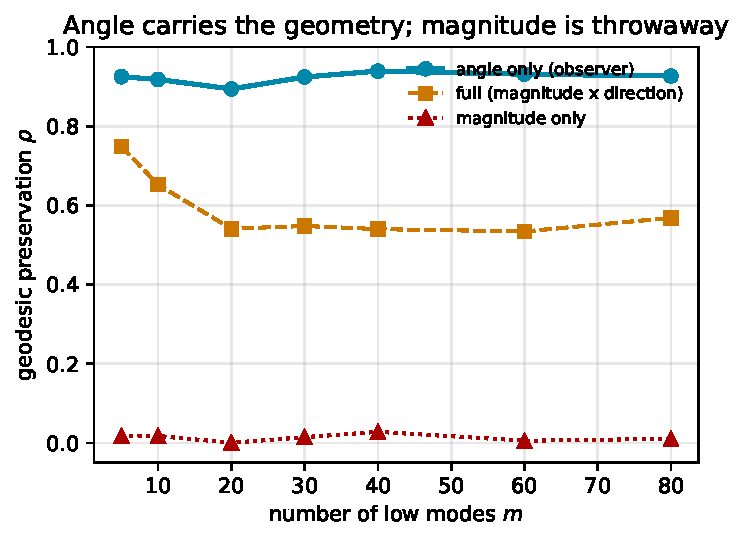
\includegraphics[width=\linewidth]{fig1_core.pdf}
\caption{Spearman correlation with graph geodesics on a 2-torus
($n=2000$) versus mode-count $m$. Angle carries the geometry; magnitude carries
little geodesic signal; the full commute embedding decays with $m$.}
\label{fig:core}
\end{minipage}\hfill
\begin{minipage}[t]{0.49\linewidth}
\centering
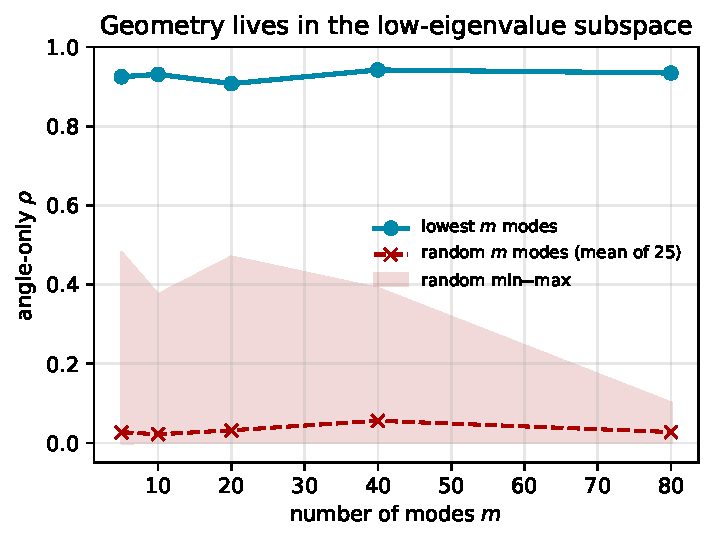
\includegraphics[width=\linewidth]{fig2_control.pdf}
\caption{Geometry lives in the low-eigenvalue subspace: lowest-$m$ modes preserve
geodesics; a random-mode basis of equal size does not. The random curve is the
mean over $25$ draws, the band its full min--max envelope---even the best-case
random draw stays far below the low-mode curve.}
\label{fig:control}
\end{minipage}
\end{figure}

\subsection{\texorpdfstring{Verifying Corollary~\ref{thm:radial} and
Conjecture~\ref{conj:angle}}{Verifying the degeneracy corollary and the angular
conjecture}}\label{sec:verify}
We check the two claims directly. The angle-$\rho$ is flat in graph size
while the full commute distance decays, and
the truncated radius tracks degree ($\rho(\lVert\Psi_i\rVert,1/\sqrt{k_i})=
0.79$--$0.87$ across $m=5$--$40$; radius-only $\rho\le0.08$). For the full
\emph{unnormalized} commute radius the degeneracy is exact,
Corollary~\ref{thm:radial} holding cleanly
at $d=3$ ($\rho(R,1/k_i+1/k_j)\to0.98$); $d=2$ is borderline (log corrections);
the quasi-1D case correctly shows no degeneracy, as the dimension gating
predicts. Conjecture~\ref{conj:angle}: in an $m$-sweep at $n=4000$, angle-$\rho$
is flat $\approx0.93$ across $m=5$--$80$ while the full embedding decays
$0.773\to0.437$.

\subsection{Which weighting carries the angle?}\label{sec:ablation}
The direction depends on the per-mode weight, so we ablate it on the torus
($d{=}2$) and a $3$-torus ($d{=}3$). Plain eigenmaps ($w_k{=}1$) give an angle
that \emph{collapses} with mode count---angle-$\rho$ falls from $0.554\pm0.013$ at
$m{=}10$ to $0.081\pm0.012$ at $m{=}20$ (five independent draws, $d{=}2$)---because
equal weighting lets high modes swamp the direction. The commute weight
$1/\sqrt{\lambda_k}$ is flat instead ($0.918\pm0.006\to0.896\pm0.006$), as is
diffusion $e^{-\lambda_k t}$; both suppress high modes,
which is what the geometry needs. The ``flat in $m$'' property is thus a property
of the weighting, not of angles in general---and it selects the commute (or
diffusion) weight, not the plain eigenmap. Proposition~\ref{prop:plain} now
supplies the continuum mechanism: plain angular distances concentrate at
$\sqrt2$ with only an oscillatory, geometry-blind correction, while the
commute correction is the (low-pass, Green-type) kernel that carries the
ranks. Degree correction, by contrast, is
\emph{invisible} to the angle: dividing or multiplying each row by $\sqrt{k_i}$
(the diffusion-map convention and its opposite) leaves angle-$\rho$ unchanged to
three digits ($0.889$ either way), because a per-node radial factor cancels under
row-normalization---a direct confirmation that the degree lives in the radius
(Corollary~\ref{thm:radial}), not the angle.

\section{Discussion and Conclusion}\label{sec:disc}
\textbf{The primary result is basis-level and substrate-agnostic.} The angular
coordinate of the low-Laplacian embedding preserves geodesics while the radial
coordinate is degree/density nuisance---von~Luxburg-degenerate for the full,
unnormalized commute radius at $d\ge3$ (Corollary~\ref{thm:radial}), and
empirically degree-tracking for the truncated, normalized radius actually in use
(\S\ref{sec:verify}). This gives Ng--Jordan--Weiss
row-normalization a geodesic justification complementary to the cluster-separation
theory of \cite{schiebinger2015}, and places it in the same scale-from-direction
decomposition that recurs in vector and KV-cache compression \cite{polarquant2025}
---the quotient, not the discard, being what recurs. The empirical reach of the
basis across substrate families, its role as a manifold diagnostic, the compression
scope boundary (angular quantization fails for attention keys, where scale is
signal, not nuisance---condition (A2) of Theorem~\ref{thm:transfer}), and a scoped
physical interpretation are developed in the companion Paper~I.b~\cite{paperIb}.

\paragraph{Open problems.} Proving Conjecture~\ref{conj:angle} (rank form, and the
bi-Lipschitz strengthening) is now reduced, at fixed $m$, to the chart hypotheses
(H1)--(H3) plus a distance-ratio condition for rank (Corollary~\ref{cor:global},
Proposition~\ref{prop:rank}); the open core is the \emph{scale-dependent} commute
uniformity---fixed-scale uniformity in $m$ is proven for the heat filter and
refuted for the commute filter (Theorem~\ref{thm:heat},
Proposition~\ref{prop:weyl})---and graph transfer at growing spectral windows
(Appendix~\ref{app:uniform}). Beyond the flat torus, where
Corollary~\ref{cor:torus} settles them, (H1)--(H3) must be checked directly---the
obstruction being the normalized upper bound, not the differential lower bound,
which never collapses (Proposition~\ref{prop:sigmamin}). Also open: extending Corollary~\ref{thm:radial} to
the truncated, normalized radius used in practice; synthesizing clean manifolds
above $d\approx2$; a dimension-adaptive basis that tunes mode-count and diffusion
time against the fidelity decay; and whether the diagnostic transfers to learned
representations (a preliminary probe is in the repository). Two directions merit an
explicit flag. The rank limit is proved for $d\le3$; at $d\ge4$ the commute Green
kernel ceases to be Hilbert--Schmidt stable (Proposition~\ref{prop:phase}), so
extending the angular-transfer guarantee to higher-dimensional manifolds requires a
stronger filter ($\mu_k^{-s/2}$, $s>d/4$) or localized spectral regularization to
prevent tangential collapse. And the radial degeneracy analyzed here parallels the
\emph{oversmoothing} pathology of deep graph neural networks, where node
representations collapse to indistinguishable points; the angular-preservation view
suggests projecting learned GNN features onto a directional basis as a comparable
mitigation.

\paragraph{Reproducibility.} The confirming experiments of this paper---the torus
core result and controls, the theorem verification, the weighting ablation, and the
truncation/normalization checks---are fully reproducible locally
(NumPy/SciPy/NetworkX, CPU), each script emitting the exact committed result JSON in
the accompanying repository, \url{https://github.com/ahb-sjsu/the-angular-observer}
(pre-registered as \texttt{PREREG\_RUNG3/4} with dated amendments). The extended
empirical program and its reproducibility tiers are documented in the companion
Paper~I.b~\cite{paperIb}.

\appendix
\section{Proof of Corollary~\ref{thm:radial}}\label{app:radial}

The diagonal statement $L^+_{ii}\to1/k_i$ does not follow from the pairwise
resistance limits alone:
$R(i,j)=L^+_{ii}+L^+_{jj}-2L^+_{ij}$ fixes only those combinations, so a
summation argument must control the error it accumulates. Two inputs are used,
both explicit in the corollary's statement: \textbf{(i)} the \emph{uniform
multiplicative} form of the
von~Luxburg--Radl--Hein degeneracy---for $d\ge3$ graphs in their model there is
a sequence $\eta_n\to0$ with
\[
R(i,j)=\Big(\frac1{k_i}+\frac1{k_j}\Big)\,(1+\eta_{ij}),\qquad
\sup_{i\ne j}\lvert\eta_{ij}\rvert\le\eta_n
\]
(this multiplicative-uniform form is not stated verbatim by \cite{vonluxburg2014}
(their Corollaries~8--9 and Propositions~29--30):
they prove an \emph{additive} deviation bound on the rescaled commute distance,
uniform over $i\ne j$, together with two-sided degree bounds; dividing the
additive bound by $1/k_i+1/k_j$ and using the degree bounds yields the displayed
$\eta_n$); and \textbf{(ii)} a bounded degree ratio,
$k_{\max}/k_{\min}\le K$ for all $n$ (their graph models satisfy this with high
probability). Write $S:=\sum_j 1/k_j$ and note $S/n\le1/k_{\min}\le K/k_i$ for
every $i$ by (ii).

\emph{Step 1 (row sums).} $L^+$ annihilates constants ($L\mathbf1=0$ and
$L^+$ shares the range of $L$ on $\mathbf1^\perp$), so $\sum_j L^+_{ij}=0$: the
gauge. Summing $R(i,j)$ over $j\ne i$ and using the gauge,
\[
\sum_{j\ne i}R(i,j)
=(n-1)L^+_{ii}+\big(\operatorname{tr}L^+-L^+_{ii}\big)
-2\sum_{j\ne i}L^+_{ij}
=n\,L^+_{ii}+\operatorname{tr}L^+,
\]
since $\sum_{j\ne i}L^+_{ij}=-L^+_{ii}$. By (i) the same sum equals
\[
\sum_{j\ne i}\Big(\frac1{k_i}+\frac1{k_j}\Big)(1+\eta_{ij})
=\frac{n-2}{k_i}+S+e_i,
\qquad
\lvert e_i\rvert\le\eta_n\Big(\frac{n}{k_i}+S\Big).
\]
Equating and dividing by $n$,
\begin{equation}
L^{+}_{ii}=\frac1{k_i}+C_n-\frac{2}{n k_i}+\frac{e_i}{n},
\qquad
C_n:=\frac{S-\operatorname{tr}L^+}{n}\ \text{ (independent of $i$)} .
\tag{A.1}
\end{equation}

\emph{Step 2 (trace identity kills $C_n$).} Summing (A.1) over $i$:
$\operatorname{tr}L^+=S+nC_n-\tfrac2nS+\tfrac1n\sum_i e_i$. Substituting
$nC_n=S-\operatorname{tr}L^+$ and solving,
\[
\operatorname{tr}L^+=S\Big(1-\frac1n\Big)+\frac{1}{2n}\sum_i e_i,
\qquad\text{hence}\qquad
C_n=\frac{S}{n^2}-\frac{1}{2n^2}\sum_i e_i .
\]
Since $\lvert\sum_i e_i\rvert\le\eta_n\sum_i(n/k_i+S)=2\eta_n nS$, we get
$\lvert C_n\rvert\le S/n^2+\eta_n S/n\le(1/n+\eta_n)\,K/k_i$ for every $i$,
using (ii).

\emph{Step 3 (conclusion).} Feeding the bounds on $C_n$ and $e_i/n$ back into
(A.1),
\[
\Big\lvert L^+_{ii}-\frac1{k_i}\Big\rvert
\ \le\ \frac{(1/n+\eta_n)K}{k_i}+\frac{2}{nk_i}
+\frac{\eta_n}{k_i}\big(1+K\big)
\ \le\ \frac{C(K)\,\big(\eta_n+1/n\big)}{k_i},
\]
so $k_iL^+_{ii}\to1$ uniformly over nodes, i.e.\
$L^+_{ii}=(1/k_i)(1+o(1))$ and $\lVert\Phi_i\rVert=\sqrt{L^+_{ii}}
=(1/\sqrt{k_i})(1+o(1))$. \hfill$\qed$

Without (ii) the conclusion weakens gracefully: the same computation gives
$L^+_{ii}=1/k_i+O\big((\eta_n+1/n)\,S/n\big)$, an \emph{additive} error at the
harmonic-mean-degree scale, so the degeneracy survives at the pairwise level
($R\approx1/k_i+1/k_j$, which is (i)) even when per-node relative control is lost.
The $j{=}i$ term ($R(i,i)=0$ while $1/k_i+1/k_j=2/k_i$) is excluded from the sums,
which is why the $(n-2)/k_i$ bookkeeping appears.


\section{Proof of Theorem~\ref{thm:cond}}\label{app:proof}

\subsection*{Setting and notation}
$M$ is a compact $d$-dimensional Riemannian manifold without boundary, volume
normalized to $1$; $(\mu_k,\varphi_k)_{k\ge0}$ are the eigenpairs of its
(positive) Laplace--Beltrami operator, $0=\mu_0<\mu_1\le\mu_2\le\cdots$, with
$\{\varphi_k\}$ orthonormal in $L^2(M)$. Under non-uniform sampling with an
admissible density the identical argument runs against the density-weighted
operator that the graph Laplacian actually converges to
\cite{garciatrillos2018,calder2022} (the $\alpha{=}1$ normalization of
Paper~I.b restores the geometric operator), with (H1)--(H2) read for
its eigenpairs. The continuum objects are
\[
F(x)=\Big(\tfrac{\varphi_k(x)}{\sqrt{\mu_k}}\Big)_{k=1}^{m},\qquad
R(x)=\lVert F(x)\rVert,\qquad N(x)=F(x)/R(x),
\]
and $m$ sits at a spectral gap: $\mu_m<\mu_{m+1}$. Write
$\Phi_m:=\max_{k\le m}\lVert\varphi_k\rVert_\infty<\infty$ (eigenfunctions on a
smooth compact manifold are smooth). The sample is $x_1,\dots,x_n$ i.i.d.\ from
the stated density class, $G_n$ the $\varepsilon$-graph (or $k$-NN graph) on it,
and $(\lambda_k,v_k)$ the eigenpairs of $L_{\mathrm{sym}}$ with the empirical
normalization $\tfrac1n\sum_i v_k(i)^2=1$; the algorithm forms
$\Psi_i=(v_k(i)/\sqrt{\lambda_k})_{k=1}^m$ and
$\hat u_i=\Psi_i/\lVert\Psi_i\rVert$. Alongside these, the \emph{random-walk}
eigenvectors $v^{\mathrm{rw}}_k:=D^{-1/2}v_k$ are the eigenpairs of
$L_{\mathrm{rw}}=D^{-1}(D-A)=D^{-1/2}L_{\mathrm{sym}}D^{1/2}$ at the \emph{same}
eigenvalue $\lambda_k$; we take them with the coordinated normalization
$\tfrac1n\sum_i k_i\,v^{\mathrm{rw}}_k(i)^2=1$ (the empirical degree-weighted inner
product---which is \emph{identically} the algorithm's own $L_{\mathrm{sym}}$
constraint $\tfrac1n\sum_i v_k(i)^2=1$ viewed through $D^{1/2}$), under which each
$v^{\mathrm{rw}}_k$ pairs mode-for-mode with the continuum eigenfunction
$\varphi_k$ orthonormal in the effective sampling measure (exactly $L^2(\rho)$ for
uniform sampling or after the $\alpha{=}1$ reweighting of Paper~I.b that
restores the geometric operator; the $\rho$-versus-$\rho^2$ distinction under raw
non-uniform sampling is immaterial, $v^{\mathrm{rw}}_k$ being only an intermediary
to the identical angular map)---the convention in which the $\infty$-norm
eigenvector rates below hold. Write
$\Psi^{\mathrm{rw}}_i=(v^{\mathrm{rw}}_k(i)/\sqrt{\lambda_k})_{k=1}^m$.

\subsection*{Step 0: three invariances}
The claim concerns only the pairwise distances $\lVert\hat u_i-\hat u_j\rVert$.
These are invariant under (i) a global rescaling of all eigenvectors (the choice
of normalization), (ii) a global rescaling of all eigenvalues (which rescales
every weight $1/\sqrt{\lambda_k}$ by the same factor), and (iii) a fixed
orthogonal transformation $Q\in O(m)$ applied to every $\Psi_i$ (then
$\lVert Q\hat u_i-Q\hat u_j\rVert=\lVert\hat u_i-\hat u_j\rVert$). We use (i) to
work in the empirical normalization, (ii) to apply the deterministic
graph-to-continuum eigenvalue scaling $c_n$ of \cite{calder2022}, and (iii) to
absorb the basis alignment of Lemma~\ref{lem:transfer}.

\smallskip\noindent\emph{(iv) Exact per-node degree cancellation.} Since
$v_k=D^{1/2}v^{\mathrm{rw}}_k$ applies the \emph{same} node factor $\sqrt{k_i}$ in
every mode $k$, the two commute-weighted embeddings differ only by a positive
per-node scalar,
\[
\Psi_i=\big(v_k(i)/\sqrt{\lambda_k}\big)_{k=1}^m
=\sqrt{k_i}\,\big(v^{\mathrm{rw}}_k(i)/\sqrt{\lambda_k}\big)_{k=1}^m
=\sqrt{k_i}\;\Psi^{\mathrm{rw}}_i ,
\]
so row normalization returns the \emph{identical} angular map
$\hat u_i=\Psi^{\mathrm{rw}}_i/\lVert\Psi^{\mathrm{rw}}_i\rVert$---exactly, with no
degree-ratio hypothesis. We may therefore calibrate the random-walk embedding
$\Psi^{\mathrm{rw}}_i$, whose $\infty$-norm convergence to the continuum is
exactly the cited theorem, and read off the angle the algorithm computes from
$L_{\mathrm{sym}}$. This is what lets the theorem hold under non-uniform sampling:
the node-dependent degree factor a symmetric calibration would have to control is
cancelled by the normalization, not bounded.

\subsection*{Step 1: the continuum angular map is locally bi-Lipschitz}
\begin{lemma}\label{lem:contang}
Under \textup{(H1)--(H2)}, for all $x,y\in M$ with $d_M(x,y)\le r_0$,
\[
a\,d_M(x,y)\ \le\ \lVert N(x)-N(y)\rVert\ \le\ b\,d_M(x,y),\qquad
a:=\frac{\sqrt{L_0^{-2}-\Lambda_0^2}}{\rho^+},\quad b:=\frac{L_0}{\rho^-}.
\]
\end{lemma}
\begin{proof}
Apply the identity of Lemma~\ref{lem:norm} to $u=F(x)$, $v=F(y)$. By (H1),
$L_0^{-2}d_M^2\le\lVert F(x)-F(y)\rVert^2\le L_0^2\,d_M^2$; by (H2),
$(R(x)-R(y))^2\le\Lambda_0^2\,d_M^2$ and $(\rho^-)^2\le R(x)R(y)\le(\rho^+)^2$.
The ratio in the identity is therefore at least
$(L_0^{-2}-\Lambda_0^2)\,d_M^2/(\rho^+)^2$---positive precisely because
$\Lambda_0<1/L_0$---and at most $L_0^2\,d_M^2/(\rho^-)^2$.
\end{proof}

Note $a\le b$: a two-sided constant satisfies $L_0^{-1}\le L_0$, so $L_0\ge1$,
hence $\sqrt{L_0^{-2}-\Lambda_0^2}\le L_0^{-1}\le L_0$, and $\rho^-\le\rho^+$.

\subsection*{Step 2: normalization is stable}
\begin{lemma}\label{lem:normstab}
For nonzero $u,w\in\mathbb{R}^m$,
\[
\Big\lVert \frac{u}{\lVert u\rVert}-\frac{w}{\lVert w\rVert}\Big\rVert
\ \le\ \frac{2\,\lVert u-w\rVert}{\max(\lVert u\rVert,\lVert w\rVert)}.
\]
\end{lemma}
\begin{proof}
$\frac{u}{\lVert u\rVert}-\frac{w}{\lVert w\rVert}
=\frac{u-w}{\lVert u\rVert}
+w\Big(\frac{1}{\lVert u\rVert}-\frac{1}{\lVert w\rVert}\Big)$, and the second
term has norm $\big|\lVert w\rVert-\lVert u\rVert\big|/\lVert u\rVert
\le\lVert u-w\rVert/\lVert u\rVert$. So the left side is at most
$2\lVert u-w\rVert/\lVert u\rVert$; by symmetry in $u\leftrightarrow w$, also at
most $2\lVert u-w\rVert/\lVert w\rVert$.
\end{proof}

\subsection*{Step 3: sup-norm spectral transfer}
This is the step for which $L^2$ consistency \cite{garciatrillos2018} does not
suffice and the $\infty$-norm rates of \cite{calder2022} are the right tool.
Group $\mu_1\le\cdots\le\mu_m$ into blocks of equal eigenvalues (multiplets);
because $m$ sits at a spectral gap, the last block ends exactly at $m$.

\smallskip\noindent Throughout this step the calibration is carried out on the
\emph{random-walk} eigenvectors: to keep notation light we drop the superscript
and write $v_k,\Psi_i,\widetilde\Psi_i$ for $v^{\mathrm{rw}}_k$ and the
corresponding random-walk commute embeddings. By invariance~(iv) the resulting
angle is exactly the algorithm's $\hat u_i$, and the $\infty$-norm rates of
\cite{calder2022}---stated for the unnormalized/random-walk eigenvectors---apply
to $v_k$ directly, with no degree-ratio hypothesis.

\begin{lemma}[Calibration; external sup-norm transfer]\label{lem:transfer}
Under the sampling model of \cite{calder2022,calderlewicka2022} there are sequences
$\epsilon_n,\delta_n\to0$---the eigenvector $L^\infty$ rate of
\cite{calderlewicka2022} (which establishes high-probability $L^\infty$ and
$C^{0,1}$ convergence of graph Laplacian eigenvectors to the Laplace--Beltrami
eigenfunctions, with constants depending on the eigenvalue $\mu_m$ and hence on
$m$; $\epsilon_n$ carries a factor $\sqrt m$), and the eigenvalue and
gap-stability rate $\delta_n$ of \cite{calder2022}---and events $\mathcal A_n$
with $\mathbb P(\mathcal A_n)\to1$ on which, after the eigenvalue scaling
$\tilde\lambda_k:=\lambda_k/c_n$ of invariance (ii), there is an orthogonal
$Q_n\in O(m)$, block-diagonal across the multiplets, with
\[
\max_{k\le m}\big|\tilde\lambda_k-\mu_k\big|\le\delta_n,
\qquad
\max_{i\le n}\big\lVert Q_n v(i)-\varphi(x_i)\big\rVert\le\epsilon_n,
\]
where $v(i)=(v_1(i),\dots,v_m(i))$ and
$\varphi(x)=(\varphi_1(x),\dots,\varphi_m(x))$. Consequently, with
$\widetilde\Psi_i:=\big(v_k(i)/\sqrt{\tilde\lambda_k}\big)_{k=1}^m$ (the same
angle as $\Psi_i$, by invariances (i),(ii),(iv)) and provided $\delta_n\le\mu_1/2$,
\[
\max_{i\le n}\ \big\lVert Q_n\widetilde\Psi_i-F(x_i)\big\rVert\ \le\ E_n
:=\frac{\epsilon_n}{\sqrt{\mu_1}}
+\frac{2\delta_n}{\mu_1^{3/2}}\,\sqrt m\,\big(\Phi_m+\epsilon_n\big)
\ \longrightarrow\ 0 .
\]
In particular the graph radius inherits the continuum band:
$\rho^--E_n\le\lVert\widetilde\Psi_i\rVert\le\rho^++E_n$ for every node $i$.
\end{lemma}

\begin{proof}
\emph{(a) Spectral consistency.} For the unnormalized and random-walk graph
Laplacians, \cite{calder2022} give, with probability tending to one, eigenvalue
convergence $|\tilde\lambda_k-\mu_k|\le\delta_n$ and the gap stability that makes
``fixed $m$ at a spectral gap'' well-posed, while \cite{calderlewicka2022}
supplies the eigenvector consistency in $\infty$-norm with explicit rates (and an
approximate $C^{0,1}$/gradient rate $\epsilon_n'\to0$ for the eigenvectors
themselves, used for the cutoff in the remark below), stated per eigenvalue
cluster. We make the block-orthogonal alignment explicit, since
\cite{calderlewicka2022} (Theorem~2.6 with Remark~2.8) attaches to each discrete
eigenvector $v_k$ a
\emph{single} normalized limit eigenfunction $\tilde\varphi_k$ (their sup-norm
rate, $\lVert v_k-\tilde\varphi_k\rVert_\infty\lesssim\mu_k\varepsilon_n$), not an
orthonormal eigenspace basis. Within a multiplet the partners
$\{\tilde\varphi_k\}$ need not be exactly orthonormal, but their \emph{population}
Gram matrix $G=\big(\langle\tilde\varphi_k,\tilde\varphi_l\rangle_{L^2(\rho)}\big)$
is $I+O(\varepsilon_n)$, routed through the discrete vectors: the $v_k$ are
orthonormal in the empirical inner product ($\tfrac1n\sum_i v_k(i)v_l(i)=\delta_{kl}$),
each $\tilde\varphi_k$ is sup-norm $\varepsilon_n$-close to $v_k$ on the sample, and
empirical inner products concentrate on their $L^2(\rho)$ values at the
eigenvector-consistency rate, so
$\langle\tilde\varphi_k,\tilde\varphi_l\rangle_{L^2(\rho)}=\delta_{kl}+O(\varepsilon_n)$. Symmetric orthogonalization
$G^{-1/2}=I+O(\varepsilon_n)$ therefore turns $\{\tilde\varphi_k\}$ into an exactly
$L^2(\rho)$-orthonormal basis of the limiting eigenspace at cost $O(\varepsilon_n)$
in sup-norm; the alignment of this basis to the reference eigenbasis
$\{\varphi_k\}$ is the \emph{unique} block rotation $Q_n\in O(m)$ (block-diagonal
across multiplets, the orthogonal factor in the polar decomposition of the
cross-Gram $\langle\tilde\varphi_k,\varphi_l\rangle$)---not $G^{-1/2}$ itself, which
is symmetric positive-definite. Each aligned discrete eigenvector is then
$(\epsilon_n/\sqrt m)$-close in sup-norm to its partner. (Multiplicity is exactly why the alignment is block-orthogonal rather
than a per-mode sign choice; a simple eigenvalue is the $1\times1$ block, where it
\emph{is} a sign choice.) Collecting the $m$ per-mode bounds into the vector $v(i)$
gives $\lVert Q_nv(i)-\varphi(x_i)\rVert\le\epsilon_n$.

\emph{(b) No normalization conversion is needed.} The calibration in (a) is for
the random-walk eigenvectors, and by the exact per-node cancellation of
Step~0\,(iv) the graph angular map is
$\hat u_i=\Psi^{\mathrm{rw}}_i/\lVert\Psi^{\mathrm{rw}}_i\rVert$ regardless of
whether $L_{\mathrm{sym}}$ or $L_{\mathrm{rw}}$ is diagonalized: the algorithm's
embedding satisfies $\Psi_i=\sqrt{k_i}\,\Psi^{\mathrm{rw}}_i$ and the positive
scalar $\sqrt{k_i}$ cancels under row normalization. In particular no uniform
degree concentration is invoked and no bound on the degree ratio $k_i/\bar k_n$
is required, so the transfer is valid under non-uniform sampling; the sampling
density enters only by fixing the limiting (weighted) operator whose
eigenfunctions $\varphi_k$ appear in $F$, as in the Setting. (The similarity
$L_{\mathrm{rw}}=D^{-1/2}L_{\mathrm{sym}}D^{1/2}$ that underlies
$v^{\mathrm{sym}}_k=D^{1/2}v^{\mathrm{rw}}_k$ is exact, so the shared eigenvalue
$\lambda_k$ used throughout is unaffected.)

\emph{(c) Bookkeeping.} Let $W_\mu=\operatorname{diag}(\mu_k^{-1/2})$ and
$\widetilde W=\operatorname{diag}(\tilde\lambda_k^{-1/2})$, so
$F(x)=W_\mu\varphi(x)$ and $\widetilde\Psi_i=\widetilde W v(i)$. Since $W_\mu$
is a scalar multiple of the identity on each multiplet and $Q_n$ is
block-diagonal across the multiplets, $Q_nW_\mu=W_\mu Q_n$. Hence
\[
Q_n\widetilde\Psi_i-F(x_i)
=Q_n\big(\widetilde W-W_\mu\big)v(i)
+W_\mu\big(Q_nv(i)-\varphi(x_i)\big).
\]
For the first term, $\delta_n\le\mu_1/2$ gives $\tilde\lambda_k\ge\mu_1/2$, so
\[
\big\lVert\widetilde W-W_\mu\big\rVert_{\mathrm{op}}
=\max_{k\le m}\frac{|\mu_k-\tilde\lambda_k|}
{\sqrt{\tilde\lambda_k\,\mu_k}\,\big(\sqrt{\tilde\lambda_k}+\sqrt{\mu_k}\big)}
\ \le\ \frac{2\delta_n}{\mu_1^{3/2}},
\]
while $\lVert v(i)\rVert\le\lVert Q_nv(i)-\varphi(x_i)\rVert
+\lVert\varphi(x_i)\rVert\le\epsilon_n+\sqrt m\,\Phi_m
\le\sqrt m\,(\Phi_m+\epsilon_n)$. For the second term,
$\lVert W_\mu\rVert_{\mathrm{op}}=\mu_1^{-1/2}$. Adding the two bounds gives
$E_n$. The radius statement is the reverse triangle inequality
$\big|\lVert\widetilde\Psi_i\rVert-R(x_i)\big|
=\big|\lVert Q_n\widetilde\Psi_i\rVert-\lVert F(x_i)\rVert\big|\le E_n$
together with $\rho^-\le R\le\rho^+$ from (H2).
\end{proof}

\emph{General filters (proof of the calibration claim in
Corollary~\ref{cor:filtered}).} The proof above uses only two properties of
the weight matrix $W_\mu=\operatorname{diag}(\mu_k^{-1/2})$: it is constant on
multiplets (hence commutes with the block-orthogonal $Q_n$), and it is
Lipschitz in the eigenvalue on the retained window. Both hold for any positive
Lipschitz filter $h$: replacing $W_\mu$ by
$H:=\operatorname{diag}(h(\mu_k))$ and $\widetilde W$ by
$\operatorname{diag}(h(\tilde\lambda_k))$, step (c) goes through verbatim with
$\lVert\operatorname{diag}(h(\tilde\lambda_k))-H\rVert_{\mathrm{op}}
\le L_h\delta_n$ and $\lVert H\rVert_{\mathrm{op}}\le H_m$, giving
$E_{n,h}=H_m\epsilon_n+L_h\delta_n\sqrt m\,(\Phi_m+\epsilon_n)$ as claimed;
the commute filter $h(\lambda)=\lambda^{-1/2}$ (with $L_h\le2\mu_1^{-3/2}$ on
$[\mu_1/2,\infty)$ and $H_m=\mu_1^{-1/2}$) recovers the $E_n$ displayed above.

\smallskip\noindent\emph{Conditional structure, and the bridge to uniformity in
$m$.} Step~3 is \emph{external}: it composes the named rate theorems
\cite{calder2022,calderlewicka2022} into the calibration, and the transfer of the
continuum bi-Lipschitz constants to the graph is then the elementary
node-uniform perturbation of Step~4 (radius floor $\lVert\widetilde\Psi_i\rVert\ge
\rho^--E_n$; angular error $\le2E_n/\rho^-$ by Lemma~\ref{lem:normstab}; cutoff
$\theta_n\asymp E_n/a$). Consequently Theorem~\ref{thm:cond} is
\textbf{unconditional in $m$ for each fixed $m$}, resting only on this standard
sup-norm spectral-transfer lemma---no self-contained spectral analysis is
re-derived here. The one $m$-dependent seam is deliberate and worth stating
plainly: the CGLewicka constants, hence $\epsilon_n$ and $\epsilon_n'$, depend on
the retained eigenfunctions' Lipschitz norms and on the spectral gap at $\mu_m$,
so the \emph{rate} at which $\theta_n\to0$ degrades as $m$ grows. Making the
transfer \emph{uniform} in $m$---and with it (H1)---is exactly the frontier of
Conjecture~\ref{conj:angle}; we delimit it sharply in the discussion after
Proposition~\ref{prop:plain}, and it is filter-specific, since the $C^{0,1}$ rate
$\epsilon_n'$ is what shrinks $\theta_n$ toward the connectivity scale (below
which the twin obstruction lives).

\subsection*{Step 4: assembly}
\begin{proof}[Proof of Theorem~\ref{thm:cond}]
Work on the event $\mathcal A_n$ of Lemma~\ref{lem:transfer}, with $n$ large
enough that $E_n<\rho^-/2$ (so $\widetilde\Psi_i\ne0$ and every $\hat u_i$ is
defined). By invariance (iii) we may compare angles through the calibrated
embedding: writing $\hat q_i:=Q_n\widetilde\Psi_i/\lVert Q_n\widetilde\Psi_i
\rVert=Q_n\hat u_i$, Lemma~\ref{lem:normstab} with $u=Q_n\widetilde\Psi_i$,
$w=F(x_i)$, and $\lVert F(x_i)\rVert\ge\rho^-$ gives
\[
\lVert\hat q_i-N(x_i)\rVert\ \le\ \frac{2E_n}{\rho^-}
\qquad\text{for every node }i .
\]
Set $\theta_n:=8E_n/(a\rho^-)\to0$, and fix a sampled pair with
$\theta_n\le d:=d_M(x_i,x_j)\le r_0$. The pairwise angular error is at most
$4E_n/\rho^-=(a/2)\,\theta_n\le(a/2)\,d$, so by Lemma~\ref{lem:contang}, the
triangle inequality, and
$\lVert\hat u_i-\hat u_j\rVert=\lVert\hat q_i-\hat q_j\rVert$,
\[
\lVert\hat u_i-\hat u_j\rVert\ \ge\ a\,d-\tfrac a2\,d\ =\ \tfrac a2\,d\ =\ A\,d,
\qquad
\lVert\hat u_i-\hat u_j\rVert\ \le\ b\,d+\tfrac a2\,d\ \le\ 2b\,d\ =\ B\,d,
\]
the last inequality using $a\le b$ (Step 1). Both bounds hold simultaneously
for \emph{all} such pairs because the calibration of Lemma~\ref{lem:transfer}
is uniform over nodes, and $\mathbb P(\mathcal A_n)\to1$.
\end{proof}

\subsection*{Step 5: from local to global (proof of Corollary~\ref{cor:global})}
\begin{proof}[Proof of Corollary~\ref{cor:global}]
The map $(x,y)\mapsto\lVert N(x)-N(y)\rVert$ is continuous ($F$ is continuous
and $R\ge\rho^->0$) and, by (H3), strictly positive on the compact set
$\{(x,y)\in M\times M: d_M(x,y)\ge r_0\}$; its minimum $c_0$ is therefore
attained and positive. Work on the event of Lemma~\ref{lem:transfer} with $n$
large enough that $E_n<\rho^-/2$ and $4E_n/\rho^-\le c_0/2$. For sampled pairs
with $\theta_n\le d_M\le r_0$, Theorem~\ref{thm:cond} gives the bounds with
$(A,B)$, hence with $(A_g,B_g)$. For sampled pairs with $d:=d_M>r_0$: the
calibration bound $\lVert\hat q_i-N(x_i)\rVert\le2E_n/\rho^-$ of Step~4 gives
\[
\lVert\hat u_i-\hat u_j\rVert
\ \ge\ \lVert N(x_i)-N(x_j)\rVert-\frac{4E_n}{\rho^-}
\ \ge\ c_0-\frac{c_0}{2}\ =\ \frac{c_0}{2}
\ \ge\ \frac{c_0}{2\operatorname{diam}M}\,d\ \ge\ A_g\,d,
\]
while unit vectors satisfy
$\lVert\hat u_i-\hat u_j\rVert\le2\le(2/r_0)\,d\le B_g\,d$.
\end{proof}

\subsection*{Step 6: the flat torus (proof of Corollary~\ref{cor:torus})}
\begin{proof}[Proof of Corollary~\ref{cor:torus}]
On $M=\mathbb{R}^2/(2\pi\mathbb{Z})^2$ with volume normalized to $1$, the
Laplace--Beltrami eigenvalues are $\lvert k\rvert^2$, $k\in\mathbb{Z}^2$: the
first nontrivial eigenvalue $\mu=1$ has multiplicity four, spanned by the
$L^2$-orthonormal functions $\sqrt2\cos x,\ \sqrt2\sin x,\ \sqrt2\cos y,\
\sqrt2\sin y$, and the next eigenvalue is $2$---so $m=4$ exhausts the first
multiplet and sits at a spectral gap. The truncated eigenmap (weights
$1/\sqrt{\mu_k}=1$) is the Clifford embedding
$F(x,y)=\sqrt2\,(\cos x,\sin x,\cos y,\sin y)$.

\emph{(H2).} $\lVert F\rVert^2=2(\cos^2x+\sin^2x)+2(\cos^2y+\sin^2y)=4$:
the radius is constant, $R\equiv2$, so $\Lambda_0=0<1/L_0$ and
$\rho^-=\rho^+=2$.

\emph{(H1), globally.} Using
$(\cos a-\cos b)^2+(\sin a-\sin b)^2=4\sin^2\!\big(\tfrac{a-b}2\big)$,
\[
\lVert F(p)-F(q)\rVert^2
=8\Big[\sin^2\tfrac{\Delta x}{2}+\sin^2\tfrac{\Delta y}{2}\Big],
\qquad \Delta x,\Delta y\in[-\pi,\pi],
\]
while $d_M(p,q)^2=\Delta x^2+\Delta y^2$. The elementary bounds
$\tfrac{2}{\pi}\lvert\delta\rvert\le2\lvert\sin(\delta/2)\rvert\le
\lvert\delta\rvert$ on $[-\pi,\pi]$ give
\[
\frac{2\sqrt2}{\pi}\,d_M(p,q)\ \le\ \lVert F(p)-F(q)\rVert\ \le\ \sqrt2\,d_M(p,q)
\qquad\text{for \emph{all} } p,q,
\]
so (H1) holds with $L_0=\sqrt2$ (indeed $L_0^{-1}=1/\sqrt2\le2\sqrt2/\pi$) and
$r_0=\operatorname{diam}M=\pi\sqrt2$.

\emph{(H3).} $N=F/2$; since the radius is constant, $N(p)=N(q)$ iff $F(p)=F(q)$
iff $e^{\mathrm i x_p}=e^{\mathrm i x_q}$ and
$e^{\mathrm i y_p}=e^{\mathrm i y_q}$ iff $p=q$.

Because $r_0=\operatorname{diam}M$, Theorem~\ref{thm:cond} alone is already
global, with $A=\sqrt{L_0^{-2}}/(2\rho^+)=1/(4\sqrt2)$ and
$B=2L_0/\rho^-=\sqrt2$. The sharp continuum distortion of $N$ is the exact
ratio range above: $\lVert N(p)-N(q)\rVert/d_M(p,q)\in[\sqrt2/\pi,\,1/\sqrt2]$,
the ratio of whose extremes is $\pi/2$, attained along a coordinate direction at
antipodal ($\lvert\delta\rvert=\pi$) and infinitesimal separations
respectively. Basis-independence: any $L^2$-orthonormal basis of the $\mu=1$
eigenspace equals $Q$ applied to the Clifford one for some $Q\in O(4)$, and
angular pairwise distances are $Q$-invariant (Step~0, invariance (iii)).
\end{proof}

\subsection*{Step 6b: the homogeneous instance (proof of Theorem~\ref{thm:takahashi})}
\begin{proof}[Proof of Theorem~\ref{thm:takahashi}]
\emph{(a) Constant radius.} The function $S(x)=\sum_k\varphi_k(x)^2$ is
independent of the chosen $L^2$-orthonormal basis of $V_\lambda$ (an $O(m)$
change of basis leaves $\sum_k\varphi_k^2$ fixed). Since $G$ acts on $M$ by
isometries it permutes eigenspaces, so $g^*V_\lambda=V_\lambda$ for every
$g\in G$, and $g$ acts on $V_\lambda$ as an $L^2$-orthogonal map; hence
$S(g\cdot x)=S(x)$. Transitivity of $G$ then forces $S\equiv r_\lambda^2$
constant, and $S>0$ because a nonzero eigenfunction cannot vanish on an open set.
So $\lVert F\rVert\equiv r_\lambda$ and $F(M)\subset r_\lambda\,S^{m-1}$: (H2)
holds with $\Lambda_0=0$, $\rho^\pm=r_\lambda$.

\emph{(b) Homothety and the bi-Lipschitz constant.} By hypothesis
$\sum_k d\varphi_k\otimes d\varphi_k=c_\lambda g$, i.e.\ for every tangent $v$,
$\lVert dF(v)\rVert^2=\sum_k(d\varphi_k(v))^2=c_\lambda\lVert v\rVert_g^2$; thus
$F$ is a similarity of constant ratio $\sqrt{c_\lambda}$ and
$N=F/r_\lambda\colon(M,g)\to S^{m-1}$ has $\lVert dN(v)\rVert^2
=(c_\lambda/r_\lambda^2)\lVert v\rVert_g^2$. Therefore $N$ is an isometric
immersion of the rescaled manifold $\big(M,(c_\lambda/r_\lambda^2)g\big)$ into the
unit sphere, and $\Delta_g\varphi_k=\lambda\varphi_k$ makes it a \emph{minimal}
immersion in Takahashi's sense \cite{takahashi1966} (the mean curvature vector of
$F$ in $\mathbb R^m$ is $-\lambda F$, normal to the sphere). Along any geodesic of
$(M,g)$ the $N$-image is a curve on $S^{m-1}$ of speed $\sqrt{c_\lambda}/r_\lambda$
times arclength, so points at geodesic separation $d_M(x,y)$ whose images subtend
spherical arc $\theta=(\sqrt{c_\lambda}/r_\lambda)\,d_M(x,y)\le\pi$ have Euclidean
chord $\lVert N(x)-N(y)\rVert=2\sin(\theta/2)$. The elementary bound
$2\sin(\theta/2)\in[\tfrac2\pi\theta,\theta]$ on $[0,\pi]$ gives the displayed
two-sided estimate, hence (H1) with $L_0=r_\lambda/\sqrt{c_\lambda}$ on the region
where $N$ is injective (globally, if $N$ embeds).

\emph{(c) The two structural sufficient conditions.} The tensor
$T:=\sum_k d\varphi_k\otimes d\varphi_k$ is basis-free and $G$-invariant (same
argument as $S$), so it is an invariant symmetric $2$-tensor. If the isotropy
representation of $K$ on $T_oM$ is $\mathbb R$-irreducible, Schur's lemma leaves a
one-dimensional space of invariant symmetric $2$-tensors, spanned by $g$; hence
$T=c_\lambda g$ and every eigenspace is $\lambda$-standard \cite{wolf1968}. For a
Riemannian product $M=M_1\times\cdots\times M_r$ of standard factors and a joint
eigenvalue, $T=\bigoplus_i c^{(i)}g_i$; when the factors are congruent (e.g.\
equal circles in $\mathbb T^d$) the $c^{(i)}$ coincide and $T=c_\lambda g$.

\emph{Instances.} On $S^d\subset\mathbb R^{d+1}$ the $\ell{=}1$ eigenspace
($\lambda=d$) has $F\propto(x_0,\dots,x_d)$, $N=\mathrm{id}$,
$c_\lambda/r_\lambda^2=1$, recovering Corollary~\ref{cor:sphere} with the sharp
$[2/\pi,1]$. On $\mathbb T^d=\mathbb R^d/(2\pi\mathbb Z)^d$ the first shell
($\lambda=1$, $m=2d$) has $F=\sqrt2(\cos x_i,\sin x_i)_i$, and
$\sum_k d\varphi_k\otimes d\varphi_k=2\sum_i dx_i^2=2g$, so $c_\lambda=2$,
$r_\lambda=\sqrt{2d}$; for $d=2$ this is the Clifford embedding of
Corollary~\ref{cor:torus} ($r_\lambda=2$). In both, $N$ is injective, so the
graph-transfer conclusion is unconditional.
\end{proof}

\subsection*{Step 7: the small-ball ratio law (used by Proposition~\ref{prop:rank})}
Let $D_1,D_2$ be i.i.d.\ with the small-ball distance law
$F(r)=(r/r_0)^d$ on $[0,r_0]$ (density $\propto r^{d-1}$, the flat
approximation to pair distances within a geodesic ball). For $\kappa\ge1$,
\[
\mathbb P\big(D_2\ge\kappa D_1\big)
=\int_0^{r_0}\!F\!\big(\tfrac{y}{\kappa}\big)\,dF(y)
=\frac{1}{\kappa^d}\int_0^{r_0}\Big(\frac{y}{r_0}\Big)^{d}\,
\frac{d\,y^{d-1}}{r_0^{d}}\,dy
=\frac{1}{2\kappa^d},
\]
so by symmetry $\mathbb P(\max/\min\ge\kappa)=\kappa^{-d}$ and
$\mu(\kappa)=1-\kappa^{-d}$ exactly. The rank certificate of
Proposition~\ref{prop:rank} is thus $\tau\ge2\kappa^{-d}-1$,
$\rho_S\ge3\kappa^{-d}-2$: exponential decay of the worst case in the
intrinsic dimension.

\subsection*{Why the resolution cutoff is necessary}
The cutoff $\theta_n$ is forced by the statement's generality, not by the
method. In a hard-threshold $\varepsilon$-graph, two sample points at distance
below the bandwidth can be \emph{combinatorial twins}---identical
neighbourhoods, hence identical rows of $A$ and equal degrees. For twins
$i,j$ the difference $e_i-e_j$ is itself an eigenvector of
$L_{\mathrm{sym}}$---at eigenvalue $1$ for non-adjacent twins and $1+1/k$ for
adjacent ones---so every eigenvector at any \emph{other} eigenvalue is
orthogonal to it and has identical entries at $i$ and $j$. In particular
every low mode does, hence $\hat u_i=\hat u_j$ exactly while
$d_M(x_i,x_j)>0$: no lower bound $A\,d_M$ can hold below the
connectivity scale. (``Identical in every eigenvector'' would be literally
false---the localized twin-difference mode itself separates them---but that
mode sits at the top of the spectrum, far above anything the angular map
retains.) What is improvable is the \emph{size} of $\theta_n$: our
proof takes it at the sup-norm consistency rate $E_n$, much larger than the
bandwidth; a $C^1$ (gradient) consistency argument---the Lipschitz regularity
theory for graph-Laplacian eigenfunctions of \cite{calderlewicka2022} is the
natural ingredient---would control eigenvector \emph{differences} at small
separations directly and could shrink $\theta_n$ toward the connectivity scale,
below which the twin obstruction is final.

Two further remarks. (1) Every constant in $E_n$ depends on the fixed
mode-count $m$ (through $\sqrt m$, $\Phi_m$, $\mu_1$, and the gap
$\mu_{m+1}-\mu_m$); nothing here is claimed uniform in $m$. The uniformity in
$m$ observed empirically (\S\ref{sec:verify}) corresponds to the
uniformity of (H1) \cite{bates2014,portegies2016} and is exactly what separates
Theorem~\ref{thm:cond} from the full Conjecture~\ref{conj:angle};
Appendix~\ref{app:uniform} settles its continuum side by filter (uniform for
heat, scale-dependent for commute). (2) The
theorem is local ($d_M\le r_0$) because (H1) is; the global statement needs
precisely the injectivity hypothesis (H3), which Corollary~\ref{cor:global}
(Step~5) carries out---and on the flat torus (H1) is itself global, so
Corollary~\ref{cor:torus} (Step~6) needs none of (H1)--(H3).

\section{Uniformity in the truncation}\label{app:uniform}

This appendix proves Theorem~\ref{thm:heat} and Proposition~\ref{prop:weyl},
and records the growing-window graph-transfer conditions. Throughout, volume
is normalized to $1$, $p_t$ is the heat kernel of $M$, and cutoffs are
multiplet-closed.

\subsection*{Proof of Theorem~\ref{thm:heat}}
Let $F_t(x)=\big(e^{-t\mu_k/2}\varphi_k(x)\big)_{k\ge1}\in\ell^2$ be the
\emph{full} heat embedding with the constant mode removed; its kernel is
\[
K_t(x,y):=\langle F_t(x),F_t(y)\rangle=p_t(x,y)-1 .
\]

\emph{Step 1: $N_t$ is a uniformly noncollapsing immersion for small $t$.}
For a unit tangent vector $v\in T_xM$,
\[
\lVert dF_t(v)\rVert^2=\partial^v_x\partial^v_y K_t(x,y)\big|_{y=x},
\qquad
dR_t(v)=\frac{\partial_v K_t(x,x)}{2R_t(x)},
\qquad R_t^2(x)=p_t(x,x)-1 .
\]
By the Minakshisundaram--Pleijel expansion (cf.\ \cite{berard1994}),
$p_t(x,x)=(4\pi t)^{-d/2}\big(1+t\,\mathrm{scal}(x)/6+O(t^2)\big)$ and
$\partial^v_x\partial^v_y p_t\big|_{y=x}=\tfrac1{2t}(4\pi t)^{-d/2}(1+O(t))$,
both uniformly on compact $M$. The only $x$-dependence of the diagonal at this
order is through the curvature term, so
$\partial_v p_t(x,x)=(4\pi t)^{-d/2}\,O(t)$, whence
$dR_t(v)^2=(4\pi t)^{-d/2}\,O(t^{2})\cdot O(1)$, which is $o$ of the
derivative energy $\asymp t^{-1}(4\pi t)^{-d/2}$. Therefore there is
$t_0(M)>0$ such that for $t\le t_0$ the tangential square
$T_t(x,v)^2:=\lVert dF_t(v)\rVert^2-dR_t(v)^2$ obeys
\[
T_t(x,v)^2\ \ge\ c\,t^{-d/2-1},\qquad
R_t(x)^2\asymp t^{-d/2},\qquad\text{hence}\qquad
\lVert dN_t(v)\rVert^2=\frac{T_t(x,v)^2}{R_t(x)^2}\ \ge\ \frac{c'}{t},
\]
uniformly over the unit tangent bundle (the last identity is
Proposition~\ref{prop:angdist}).

\emph{Step 2: the truncation tail vanishes in $C^2$.} Eigenfunction
H\"older/derivative norms grow only polynomially,
$\lVert\varphi_k\rVert_{C^r}\le C\mu_k^{(d-1)/4+r/2}$ \cite{hormander1968},
while the heat weights decay exponentially; hence
$\lVert F_t-F_{t,m}\rVert_{C^2}\to0$ as $m\to\infty$ (tail sums
$\sum_{k>m}e^{-t\mu_k}\mu_k^{c(d,r)}\to0$ by Weyl's law). Consequently
$T_{t,m}\to T_t$, $R_{t,m}\to R_t$, and the $C^2$-norms of $N_{t,m}$ converge,
all uniformly; choose $m_0(t)$ so that for $m\ge m_0(t)$,
$T_{t,m}^2\ge\tfrac12c\,t^{-d/2-1}$, $R_{t,m}\asymp t^{-d/4}$, and
$\sup_{m\ge m_0}\lVert N_{t,m}\rVert_{C^2}=:C_2(t)<\infty$.

\emph{Step 3: from uniform immersion to uniform bi-Lipschitz.} Let
$a_t':=\inf_{m\ge m_0}\inf_{x,\lvert v\rvert=1}\lVert dN_{t,m}(v)\rVert>0$
from Steps 1--2. For $x,y$ with $d:=d_M(x,y)\le r_t:=a_t'/(2C_2(t))$, Taylor
along a minimizing geodesic $\gamma$ gives
\[
\lVert N_{t,m}(x)-N_{t,m}(y)\rVert
\ \ge\ \lVert dN_{t,m}(\gamma'(0))\rVert\,d-\tfrac12C_2(t)\,d^2
\ \ge\ \Big(a_t'-\tfrac12C_2(t)\,r_t\Big)d\ \ge\ \tfrac{3a_t'}{4}\,d,
\]
and the mean-value bound gives
$\lVert N_{t,m}(x)-N_{t,m}(y)\rVert\le b_t\,d$ with
$b_t:=\sup_{m\ge m_0}\mathrm{Lip}(N_{t,m})<\infty$. All constants depend on
$t$ and $M$ only---not on $m$. \hfill$\qed$

\begin{lemma}[Differentiated pointwise Weyl law]\label{lem:dweyl}
Let $(M,g)$ be a smooth closed Riemannian $d$-manifold with orthonormal
Laplace eigenfunctions $\varphi_k$, eigenvalues $\mu_k$. There are constants
$c_d,c_d'>0$ depending only on $(M,g)$ such that, uniformly in $x\in M$,
\[
\sum_{0<\mu_k\le\Lambda}\varphi_k(x)^2
   \;=\; c_d\,\Lambda^{d/2}\,\bigl(1+O(\Lambda^{-1/2})\bigr),
\qquad
\sum_{0<\mu_k\le\Lambda}\lVert\nabla\varphi_k(x)\rVert^2
   \;=\; c_d'\,\Lambda^{(d+2)/2}\,\bigl(1+O(\Lambda^{-1/2})\bigr),
\]
with spatially constant leading coefficients.
\end{lemma}
\begin{proof}
Both are on-diagonal statements about the spectral projector
$\Pi_\lambda(x,y)=\sum_{\sqrt{\mu_k}\le\lambda}\varphi_k(x)\varphi_k(y)$ at
frequency $\lambda=\sqrt\Lambda$: the first is H\"ormander's pointwise Weyl law
with sharp remainder \cite{hormander1968},
$\Pi_\lambda(x,x)=\tilde c_d\lambda^{d}+O(\lambda^{d-1})$; the second is the
mixed-derivative case $\partial_{x}\!\cdot\!\partial_{y}\Pi_\lambda(x,y)
\big|_{y=x}=\tilde c_d'\lambda^{d+2}+O(\lambda^{d+1})$, the uniform derivative
estimates for the spectral function on a closed manifold of \cite{binxu2004} (one
power of $\lambda$ below the main term, uniformly on $M$; no non-self-focal
restriction, which the finer scaling limit of \cite{canzanihanin2015} would
carry). Substituting $\lambda=\sqrt\Lambda$
gives the stated relative remainders.
\end{proof}

\subsection*{Proof of Proposition~\ref{prop:weyl}}
Let $E_\Lambda(x,y)=\sum_{\mu_k\le\Lambda}\varphi_k(x)\varphi_k(y)$ be the
spectral function. The pointwise Weyl law with uniform remainder
\cite{hormander1968} gives $E_\Lambda(x,x)=C_d\Lambda^{d/2}+O(\Lambda^{(d-1)/2})$
with spatially constant leading coefficient, and its differentiated form
(the uniform derivative-Weyl estimates of \cite{binxu2004}; equivalently
Lemma~\ref{lem:dweyl}) gives, uniformly in $x$ and unit $v$,
\[
\partial^v_x\partial^v_y E_\Lambda(x,y)\big|_{y=x}
=C'_d\,\Lambda^{d/2+1}\big(1+o(1)\big).
\]
Abel summation in the cutoff converts these into the commute-weighted sums:
\[
\lVert dF_\Lambda(v)\rVert^2
=\sum_{0<\mu_k\le\Lambda}\mu_k^{-1}\big(\partial_v\varphi_k(x)\big)^2
=c_d\,\Lambda^{d/2}\big(1+o(1)\big),
\]
\[
G_\Lambda(x,x):=R_\Lambda^2(x)
=\sum_{0<\mu_k\le\Lambda}\mu_k^{-1}\varphi_k(x)^2
=\begin{cases}
C_d\,\Lambda^{d/2-1}\big(1+o(1)\big), & d>2,\\[2pt]
C_2\log\Lambda\,\big(1+o(1)\big), & d=2,
\end{cases}
\]
again uniformly in $x$ (Lemma~\ref{lem:dweyl} in the commute-weighted
normalization; Abel summation in the cutoff converts the on-diagonal projector
asymptotics into the $\mu^{-1}$-weighted sums), with spatially constant leading
coefficients. Because the leading coefficient of $G_\Lambda(x,x)$ is spatially
constant, its spatial derivative has no leading term, and the differentiated
remainder estimates of \cite{binxu2004} bound what remains,
$\partial_vG_\Lambda(x,x)=o(\Lambda^{(d-1)/2})$ uniformly---weaker than the naive
$o(\Lambda^{d/2-1})$ and all that is needed---so the radial term
$dR_\Lambda(v)^2=\big(\partial_vG_\Lambda(x,x)\big)^2/\big(4G_\Lambda(x,x)\big)
=o(\Lambda^{d/2})$ is lower order than the derivative energy. Hence
$T_\Lambda(x,v)^2\ge c\,\Lambda^{d/2}$ for $\Lambda\ge\Lambda_0$, uniformly,
which is the display; dividing by $R_\Lambda^2$ gives
$\lVert dN_\Lambda\rVert\gtrsim\Lambda^{1/2}$ ($d>2$) and
$\sqrt{\Lambda/\log\Lambda}$ ($d=2$).

\emph{The $S^1$ computation, and the failure of fixed-scale uniformity.} On
$S^1$ ($\mu=k^2$, whole eigenspaces, weights $\mu^{-1/2}=1/k$),
\[
F_N(x)=\Big(\tfrac{\cos kx}{k},\tfrac{\sin kx}{k}\Big)_{k=1}^{N}:\qquad
R_N^2=\sum_{k\le N}\frac1{k^2}\ \text{(constant, bounded)},\qquad
\lVert dF_N\rVert^2=\sum_{k\le N}1=N,
\]
so $\lVert dN_N\rVert=\lVert dF_N\rVert/R_N\asymp\sqrt N$ (consistent with the
general formula: $\Lambda=N^2$, $d=1$, $T_\Lambda/R\asymp\Lambda^{1/4}$). A
pair at distance $\sim1/N$ is stretched by $\sim\sqrt N$, so any upper
Lipschitz constant valid on a \emph{fixed} ball $\{d\le r_0\}$ must grow like
$\sqrt m$: no $m$-independent fixed-scale bi-Lipschitz theorem can hold for
the commute filter, on any manifold (the same growth holds in all $d$). The
lower bound at fixed scale, by contrast, survives on $S^1$ (project onto the
first multiplet, whose weight is $m$-independent while $R_N$ is bounded)---the
failure is one-sided and lives below the wavelength $\Lambda^{-1/2}$.
\hfill$\qed$

\begin{remark}[Cutoff-insensitivity]
The conclusion of Proposition~\ref{prop:weyl} does not depend on the sharp
spectral cutoff: replacing $\sum_{\mu_k\le\Lambda}$ by a smoothed
Littlewood--Paley weight $\chi(\mu_k/\Lambda)$ yields the same growth orders with
full asymptotic expansions (smoothed spectral sums admit wave-kernel expansions
without Tauberian remainders), and on $\mathbb S^1$ the sharp-cutoff computation
is exact with no Weyl input at all. The proposition's content---no $m$-independent
fixed-scale upper Lipschitz constant for the commute filter---is
cutoff-independent.
\end{remark}

\subsection*{A uniform lower angular bound on flat tori}
\begin{proposition}[Uniform lower angular bound on flat tori]
\label{prop:torus-lower-uniform}
Let $T=\mathbb R^d/\Gamma$ be a fixed flat torus with dual lattice $\Gamma^*$. For
a multiplet-closed spectral cutoff $\Lambda$, set
\[
F_\Lambda(x)=\Big(\tfrac{e^{i\langle\xi,x\rangle}}{\lvert\xi\rvert}\Big)_{\xi\in\Gamma^*\setminus\{0\},\ \lvert\xi\rvert^2\le\Lambda},
\qquad
N_\Lambda(x)=\frac{F_\Lambda(x)}{\lVert F_\Lambda(x)\rVert}
\]
(equivalently, pair $\xi$ with $-\xi$ and use real sine--cosine coordinates). There
exist $\Lambda_0(T)<\infty$ and $c_T>0$ such that
\[
\lVert N_\Lambda(x)-N_\Lambda(y)\rVert\ \ge\ c_T\,d_T(x,y)
\]
for every multiplet-closed $\Lambda\ge\Lambda_0(T)$ and every $x,y\in T$; the lower
angular Lipschitz constant is thus uniform in the mode count $m=m(\Lambda)$. For the
standard torus $\mathbb T^d=\mathbb R^d/(2\pi\mathbb Z)^d$ one may take $\Lambda_0=1$.
\end{proposition}

\begin{proof}
We work first on the standard torus; the general lattice is treated at the end.
Write $R=\sqrt\Lambda$ and $\mathcal K_R=\{k\in\mathbb Z^d\setminus\{0\}:\lvert k\rvert\le R\}$.
Because the cutoff contains complete sine--cosine pairs,
$S_R:=\lVert F_R(x)\rVert^2=\sum_{k\in\mathcal K_R}\lvert k\rvert^{-2}$ is
independent of $x$. If $z=x-y$ is represented in $[-\pi,\pi]^d$ then
$d_{\mathbb T^d}(x,y)=\lvert z\rvert$ and
\begin{equation}
\lVert N_R(x)-N_R(y)\rVert^2=\frac{2A_R(z)}{S_R},\qquad
A_R(z):=\sum_{k\in\mathcal K_R}\frac{1-\cos(k\cdot z)}{\lvert k\rvert^2}.
\label{eq:sm-N}
\end{equation}
We prove $A_R(z)\ge c_d\lvert z\rvert^2 S_R$ with $c_d>0$ independent of $R$.

\smallskip\noindent\emph{A Fourier-block estimate.} For $q\ge2$ and
$t\in[-\pi,\pi]$ set $a_q(t):=\tfrac1q\sum_{n=q}^{2q-1}\cos(nt)$. There is an
absolute $c>0$ with
\begin{equation}
1-\lvert a_q(t)\rvert\ \ge\ c\,\min\{1,\,q^2t^2\}.
\label{eq:sm-block}
\end{equation}
Indeed, if $U$ is uniform on $\{q,\dots,2q-1\}$ and $\phi_q(t)=\mathbb E\,e^{iUt}$,
then $\lvert a_q(t)\rvert\le\lvert\phi_q(t)\rvert$. When $q\lvert t\rvert\le1$, for an
independent copy $U'$,
\[
1-\lvert\phi_q(t)\rvert\ \ge\ \tfrac12\big(1-\lvert\phi_q(t)\rvert^2\big)
=\tfrac12\,\mathbb E\big[1-\cos((U-U')t)\big]\ \ge\ c\,q^2t^2,
\]
using $1-\cos s\ge cs^2$ for $\lvert s\rvert\le1$ and $\mathbb E(U-U')^2\asymp q^2$.
When $q\lvert t\rvert\ge1$, the exact formula
$\lvert\phi_q(t)\rvert=\lvert\sin(qt/2)\rvert/(q\lvert\sin(t/2)\rvert)$ is bounded by
a universal $\rho<1$: for bounded $q$ the ratio is $<1$ on the compact locus
$q\lvert t\rvert\ge1$, and as $q\to\infty$ it tends to $0$ unless $t\to0$, where with
$s=qt/2\ge\tfrac12$ it equals $\lvert\sin s\rvert/s<1$. This gives \eqref{eq:sm-block}.

\smallskip\noindent\emph{Lattice blocks.} Choose $j$ with
$\lvert z_j\rvert=\lVert z\rVert_\infty$. For dyadic $q$ put
$B_{q,j}=\{k\in\mathbb Z^d:q\le\lvert k_j\rvert<2q,\ \lvert k_\ell\rvert<q\ (\ell\ne j)\}$,
disjoint across dyadic $q$, with $\lvert B_{q,j}\rvert\asymp_d q^d$ and
$\lvert k\rvert^2\le(d+3)q^2$ on $B_{q,j}$. The block average of $\cos(k\cdot z)$
factors as $a_q(z_j)\prod_{\ell\ne j}b_q(z_\ell)$ with each normalized symmetric
Dirichlet sum $\lvert b_q\rvert\le1$, so by \eqref{eq:sm-block}
\[
\frac1{\lvert B_{q,j}\rvert}\sum_{k\in B_{q,j}}\big(1-\cos(k\cdot z)\big)
\ \ge\ 1-\lvert a_q(z_j)\rvert\ \ge\ c\,\min\{1,q^2z_j^2\}.
\]
With $\lvert k\rvert^2\le(d+3)q^2$, $\lvert B_{q,j}\rvert\asymp q^d$, and
$\min\{1,q^2z_j^2\}\ge\lvert z\rvert^2/(d\pi^2)$ (from $z_j^2\ge\lvert z\rvert^2/d$
and $\lvert z\rvert\le\sqrt d\,\pi$),
\[
\sum_{k\in B_{q,j}}\frac{1-\cos(k\cdot z)}{\lvert k\rvert^2}
\ \ge\ c_d\,q^{d-2}\lvert z\rvert^2.
\]
Every block with $q\le R/\sqrt{d+3}$ lies in $\mathcal K_R$; summing over dyadic $q$
in that range,
$A_R(z)\ge c_d\lvert z\rvert^2\sum_{q\ \mathrm{dyadic},\,2\le q\le R/\sqrt{d+3}}q^{d-2}$,
while a dyadic decomposition of the lattice ball gives
$S_R\le C_d\big(1+\sum_{q\ \mathrm{dyadic},\,q\le R}q^{d-2}\big)$. The two sums are
comparable for large $R$---bounded for $d=1$, $\asymp\log R$ for $d=2$,
$\asymp R^{d-2}$ for $d\ge3$---so $A_R(z)\ge c_d\lvert z\rvert^2S_R$. For the finitely
many smaller cutoffs the first multiplet already gives
$A_R(z)\ge\sum_{j}(1-\cos z_j)\ge c_d\lvert z\rvert^2$ with $S_R$ bounded, so the
bound holds for all $R\ge1$. Substituting into \eqref{eq:sm-N},
$\lVert N_R(x)-N_R(y)\rVert^2\ge c_d\lvert z\rvert^2=c_d\,d_{\mathbb T^d}(x,y)^2$.

For a general flat torus, a dual-lattice basis $b_1,\dots,b_d$ and norm equivalence
$c_T\lvert n\rvert\le\lvert\xi(n)\rvert\le C_T\lvert n\rvert$ reduce the estimate to the
standard case in angular coordinates $\theta\in[-\pi,\pi]^d$, with constants
depending on $T$; taking $\Lambda_0(T)$ large enough to contain a dual basis handles
the initial cutoffs.
\end{proof}

\noindent Together with Proposition~\ref{prop:weyl} this locates the commute
frontier exactly: $c_T\,d_T(x,y)\le\lVert N_m(x)-N_m(y)\rVert$ uniformly in $m$, while
there is \emph{no} $m$-uniform upper bound at a fixed spatial scale, since
$\lVert dN_m\rVert$ grows with the cutoff. The lower Lipschitz half of the metric
conjecture is thus proved on the reference substrate family; only the scale-dependent
upper half remains.


\begin{remark}[Exact upper-Lipschitz divergence]\label{rem:torus-upper}
The companion upper bound diverges, on $\mathbb T^d$ exactly and for every $d$.
Because $S_R$ is independent of $x$, normalization produces no radial cancellation,
so for a coordinate direction $e_j$,
\[
\lVert dN_R(e_j)\rVert^2=\frac1{S_R}\sum_{k\in\mathcal K_R}\frac{k_j^2}{\lvert k\rvert^2}
=\frac{\lvert\mathcal K_R\rvert}{d\,S_R},
\]
using $\sum_{j=1}^d k_j^2/\lvert k\rvert^2=1$ at every lattice point. With
$\lvert\mathcal K_R\rvert\asymp R^d$ and the orders of $S_R$ above,
\[
\operatorname{Lip}(N_R)\asymp
\begin{cases}
R^{1/2}, & d=1,\\
R/\sqrt{\log R}, & d=2,\\
R, & d\ge3,
\end{cases}
\]
so no $R$-independent upper Lipschitz constant exists on any fixed geodesic ball.
This is an exact obstruction, not a gap in technique, and it survives a global
output rescaling $N_R\mapsto c_RN_R$: uniform upper control forces $c_R\to0$, which
collapses the fixed-diameter image ($\operatorname{diam}\le2c_R\to0$) and destroys
the lower bound. The commute map is therefore \emph{uniformly co-Lipschitz with a
quantitatively diverging upper Lipschitz constant}; genuine two-sided uniformity
requires a faster filter---the heat weighting (Theorem~\ref{thm:heat}), or amplitude
$\lvert k\rvert^{-s}$ with $s>(d+2)/2$, for which the numerator above converges while
$S_R$ tends to a positive constant.
\end{remark}

\subsection*{A spectral-filter phase diagram}
The commute weighting is one member of the fractional family
\[
F_{\Lambda,s}(x)=\bigl(\mu_k^{-s/2}\varphi_k(x)\bigr)_{0<\mu_k\le\Lambda},
\qquad
K_{\Lambda,s}(x,y)=\sum_{0<\mu_k\le\Lambda}\mu_k^{-s}\varphi_k(x)\varphi_k(y),
\]
with commute at $s=1$, the plain eigenmap at $s=0$, and the heat weighting a
rapidly decaying alternative. Weyl's law $\mu_k\asymp k^{2/d}$ separates three regimes
by three convergence thresholds.

\begin{proposition}[Filter thresholds]\label{prop:phase}
As $\Lambda\to\infty$,
\[
\sum_k\mu_k^{-2s}<\infty\iff s>\tfrac d4,\qquad
\sum_k\mu_k^{-s}<\infty\iff s>\tfrac d2,\qquad
\sum_k\mu_k^{1-s}<\infty\iff s>\tfrac d2+1,
\]
controlling respectively: (i) the $L^2(M\times M)$ (Hilbert--Schmidt) limit of the
correction kernel $K_{\Lambda,s}$---hence stability of the rank information it carries;
(ii) the trace $\int_M\lVert F_{\Lambda,s}\rVert^2=\sum_k\mu_k^{-s}$, i.e.\ finiteness
of the radius in the infinite embedding; and (iii) the differential energy
$\int_M\lVert dF_{\Lambda,s}\rVert^2=\sum_k\mu_k^{1-s}$, i.e.\ a finite uniform upper
Lipschitz constant.
\end{proposition}

\begin{proof}
Each equivalence is Weyl's law: $\mu_k\asymp k^{2/d}$ gives $\mu_k^{-a}\asymp k^{-2a/d}$,
and $\sum_k k^{-2a/d}<\infty\iff 2a/d>1$; take $a=2s,\,s,\,s-1$. For (i), orthonormality
gives $\lVert K_{\Lambda,s}\rVert^2_{L^2(M\times M)}=\sum_{\mu_k\le\Lambda}\mu_k^{-2s}$,
Cauchy in $\Lambda$ iff the sum converges. Claims (ii)--(iii) integrate
$\lVert F\rVert^2$ and $\lVert dF\rVert^2$ over $M$.
\end{proof}

\noindent For the commute filter $s=1$ the thresholds read $d<4$, $d<2$, and $d<0$:
\begin{center}\small
\begin{tabular}{@{}lp{0.32\linewidth}l@{}}
\toprule
Property & Convergent sum & Commute ($s=1$) \\
\midrule
Rank kernel Hilbert--Schmidt stable & $\sum\mu_k^{-2}$ & holds for $d\le3$ \\
Radius finite in the limit & $\sum\mu_k^{-1}$ & only $d=1$ (diverges $d\ge2$) \\
Uniform upper Lipschitz bound & $\sum\mu_k^{0}$ & fails $\forall\,d\ge1$ \\
\bottomrule
\end{tabular}
\end{center}
This resolves three observations at once: rank stability can survive in $d=1,2,3$ (the
empirical ``flat in $m$''); the radius changes character at $d=2$
(Corollary~\ref{thm:radial}); and two-sided uniform metric control fails in every
positive dimension (Proposition~\ref{prop:weyl}, and the exact torus divergence of the
remark above). The commute filter sits at the \emph{critical} exponent for the rank
kernel, whose stability boundary is the dimension $d=4$---a sharper structural
prediction than the five-family linear trend of Paper~I.b. A filter with
$s>d/2+1$ (the heat weighting, or amplitude $\mu_k^{-s/2}$ with $s>d/2+1$) restores a
uniform two-sided bound.


\subsection*{A rank-limit theorem on flat tori ($d\le3$)}
On a flat torus the diagonal kernel $S_\Lambda=\lVert F_\Lambda(x)\rVert^2$ is
independent of $x$, so the angular distance is an exact decreasing function of a single
scalar:
\[
\lVert N_\Lambda(x)-N_\Lambda(y)\rVert^2=2-\frac{2\,G_\Lambda(x-y)}{S_\Lambda},
\qquad
G_\Lambda(z)=\sum_{0<\lvert k\rvert^2\le\Lambda}\frac{\cos(k\cdot z)}{\lvert k\rvert^2}.
\]
Because $S_\Lambda$ does not depend on the pair, the angular distances carry exactly
the reverse ranking of $G_\Lambda(x-y)$---so although every distance concentrates at
$\sqrt2$ as $\Lambda\to\infty$ (the radius diverges, $S_\Lambda\to\infty$ for
$d\ge2$), the \emph{ordering} that rank statistics read need not degenerate.

\begin{proposition}[Rank stability on flat tori]\label{prop:rank-torus}
Let $d\le3$. Then $\sum_{k\ne0}\lvert k\rvert^{-4}<\infty$, so $G_\Lambda\to G$ in
$L^2(\mathbb T^d)$, where $G$ is the zero-mean periodic Green's function. If $(X,Y)$ is
drawn from an absolutely continuous pair law (uniform sampling suffices) whose induced law of $G(X-Y)$ is atomless, then the population
Spearman and Kendall correlations between $d_{\mathbb T^d}(X,Y)$ and
$\lVert N_\Lambda(X)-N_\Lambda(Y)\rVert$ converge to those of
$\bigl(d_{\mathbb T^d}(X,Y),\,-G(X-Y)\bigr)$. On $\mathbb S^1$ the periodic Green's
function is strictly monotone in geodesic separation, so the limiting rank correlation
is exactly $1$.
\end{proposition}

\begin{proof}
$G$ has Fourier coefficients $\lvert k\rvert^{-2}$, so
$\lVert G_\Lambda-G\rVert^2_{L^2}=\sum_{\lvert k\rvert^2>\Lambda}\lvert k\rvert^{-4}\to0$
exactly when $\sum_k\lvert k\rvert^{-4}<\infty$, i.e.\ $4>d$. Hence $G_\Lambda(X-Y)\to
G(X-Y)$ in probability along the pair law. The angular distance is a fixed continuous
strictly decreasing function of $G_\Lambda(X-Y)$ (the common factor $S_\Lambda>0$ is
immaterial to order), so its ranks converge to those of $-G(X-Y)$; atomlessness of the
limit law makes the Spearman and Kendall functionals continuous there, giving
convergence. On $\mathbb S^1$, $G(\theta)=\sum_{k\ge1}\cos(k\theta)/k^2$ is strictly
decreasing on $[0,\pi]$ (its derivative $-\sum_{k\ge1}\sin(k\theta)/k=(\theta-\pi)/2<0$
there), so $-G$ is strictly increasing in the geodesic distance $\lvert\theta\rvert$
and the rank correlation is $1$.
\end{proof}

\noindent This upgrades the empirical ``flat in $m$'' (\S\ref{sec:verify}) to a
rank-stability theorem: for $d\le3$ the commute angular ranking converges to a fixed
Green-kernel ranking---exact on $\mathbb S^1$, and a computable limiting quantity on
$\mathbb T^2,\mathbb T^3$ (where $G$ is direction-dependent, so the limit is below $1$).
For $d\ge4$ the kernel is not $L^2$-stable (Proposition~\ref{prop:phase}) and no such
limit is claimed.


\subsection*{The general Green-kernel rank limit ($d\in\{2,3\}$)}
The flat-torus computation generalizes to every closed manifold of dimension $2$ or
$3$, bypassing the impossible uniform upper Lipschitz bound and isolating the exact
geometric obstruction. For independent $X,Y$ from the volume measure, define the
\emph{Green-rank coefficient} $\rho_G(M):=\rho_S\bigl(d_M(X,Y),-G_M(X,Y)\bigr)$, where
$G_M$ is the zero-mean Green kernel of the Laplace--Beltrami operator. Angular
Preservation then splits into two questions: does the truncated angular ranking
converge uniformly in $m$ to the Green-kernel ranking, and is $\rho_G(M)>0$?

\begin{theorem}[Green-kernel limit of the commute angular ranking]\label{thm:green-rank-limit}
Let $M$ be a closed connected Riemannian manifold of dimension $d\in\{2,3\}$, volume
normalized to $1$, with Laplace--Beltrami eigenpairs $(\mu_k,\varphi_k)$. At a
multiplet-closed cutoff $\Lambda$ set
$G_\Lambda(x,y)=\sum_{0<\mu_k\le\Lambda}\varphi_k(x)\varphi_k(y)/\mu_k$,
$S_\Lambda(x)=G_\Lambda(x,x)$, and
$N_\Lambda(x)=(\mu_k^{-1/2}\varphi_k(x))_{0<\mu_k\le\Lambda}/\sqrt{S_\Lambda(x)}$. Let
$(X,Y)$ have bounded density with respect to $\mathrm{vol}\otimes\mathrm{vol}$, with
the laws of $d_M(X,Y)$ and $G(X,Y)$ atomless, where
$G(x,y)=\sum_{k\ge1}\varphi_k(x)\varphi_k(y)/\mu_k\in L^2(M\times M)$. Then
\[
\rho_S\bigl(d_M(X,Y),\ \lVert N_\Lambda(X)-N_\Lambda(Y)\rVert\bigr)\ \longrightarrow\
\rho_S\bigl(d_M(X,Y),\ -G(X,Y)\bigr),
\]
and likewise for Kendall's $\tau$. Consequently, if $\rho_G(M)>0$ there are
$\Lambda_0<\infty$ and $\rho_0>0$ with
$\rho_S\bigl(d_M(X,Y),\lVert N_\Lambda(X)-N_\Lambda(Y)\rVert\bigr)\ge\rho_0$ for every
multiplet-closed $\Lambda\ge\Lambda_0$: the rank form of Angular Preservation is uniform
in the mode count beyond a finite cutoff.
\end{theorem}

\begin{proof}
Write $C_\Lambda(x,y)=\langle N_\Lambda(x),N_\Lambda(y)\rangle=
G_\Lambda(x,y)/\sqrt{S_\Lambda(x)S_\Lambda(y)}$; since
$\lVert N_\Lambda(x)-N_\Lambda(y)\rVert^2=2-2C_\Lambda(x,y)$, angular distance carries the
reverse ranking of $C_\Lambda$.
\emph{(1) Hilbert--Schmidt limit.} The $\varphi_k\otimes\varphi_k$ are orthonormal in
$L^2(M\times M)$, so $\lVert G_{\Lambda'}-G_\Lambda\rVert^2_{L^2}=
\sum_{\Lambda<\mu_k\le\Lambda'}\mu_k^{-2}$; by Weyl's law $\mu_k\asymp k^{2/d}$ this
converges iff $d<4$, so $G_\Lambda\to G$ in $L^2(M\times M)$ for $d=2,3$.
\emph{(2) The diagonal is asymptotically constant.} The uniform pointwise Weyl law
$\sum_{\mu_k\le L}\varphi_k(x)^2=c_dL^{d/2}+O(L^{(d-1)/2})$ and partial summation give,
uniformly in $x$, $S_\Lambda(x)=a_2\log\Lambda+O(1)$ ($d=2$) or
$a_3\Lambda^{1/2}+O(\log\Lambda)$ ($d=3$); writing $A_\Lambda$ for the leading term,
$\sup_x\lvert S_\Lambda(x)/A_\Lambda-1\rvert\to0$.
\emph{(3) Rescale.} $H_\Lambda:=A_\Lambda C_\Lambda=
G_\Lambda\cdot A_\Lambda/\sqrt{S_\Lambda(x)S_\Lambda(y)}\to G$ in $L^2(M\times M)$ (the
second factor $\to1$ uniformly, and $\sup_\Lambda\lVert G_\Lambda\rVert_2<\infty$).
Multiplying $C_\Lambda$ by the positive constant $A_\Lambda$ leaves ranks unchanged, so
$\operatorname{rank}\lVert N_\Lambda(X)-N_\Lambda(Y)\rVert=\operatorname{rank}(-H_\Lambda(X,Y))$.
\emph{(4) Rank convergence.} A bounded pair density carries $H_\Lambda\to G$ in $L^2$ to
convergence in probability under the law of $(X,Y)$; atomlessness of the limit makes the
distribution functions converge, and the population Spearman/Kendall identities give
$\rho_S(d_M,-H_\Lambda)\to\rho_S(d_M,-G)$.
\end{proof}

\begin{corollary}[Uniform rank preservation on two-point homogeneous spaces]\label{cor:two-point-rank}
If, in addition, $M$ is compact two-point homogeneous, then $G(x,y)=g(d_M(x,y))$ with
$g$ strictly decreasing on $(0,\operatorname{diam}M)$; hence $\rho_G(M)=1$ and
$\rho_S\bigl(d_M(X,Y),\lVert N_\Lambda(X)-N_\Lambda(Y)\rVert\bigr)\to1$, bounded below
uniformly beyond a finite cutoff. This proves the eventual uniform-in-$m$ rank form of
Conjecture~\ref{conj:angle} on $S^2,S^3,\mathbb{RP}^2,\mathbb{RP}^3$ (the circle being
the exact Fourier case above).
\end{corollary}

\begin{proof}
Two-point homogeneity makes the invariant kernel a function of geodesic distance alone.
With $A(r)$ the area density of a geodesic sphere, the zero-mean Green function satisfies
$\Delta g=-1/\operatorname{vol}M$ off the pole, i.e.\
$A(r)\,g'(r)=-1+\operatorname{vol}(M)^{-1}\int_0^r A(s)\,ds$; since
$\int_0^r A<\operatorname{vol}M$ for $r<\operatorname{diam}M$, $g'(r)<0$, so $-G$ is
strictly increasing in $d_M$ and the population rank correlation is $1$.
\end{proof}

\noindent\emph{Graph transfer of the shrinking signal.} The rank-carrying angular
fluctuation has amplitude $\asymp A_\Lambda^{-1/2}$, so the growing-window transfer
condition sharpens. With the calibration error
$E_{n,m}=\max_i\lVert Q_n\widetilde\Psi_i-F_m(x_i)\rVert$ of Appendix~\ref{app:proof} and
$R_m\asymp\sqrt{A_m}$, normalization stability gives
$\bigl\lvert A_m\langle\widehat q_i,\widehat q_j\rangle-A_m\langle N_m(x_i),N_m(x_j)\rangle\bigr\rvert
\le C\,E_{n,m}\sqrt{A_m}$. The rank-transfer condition is therefore
$E_{n,m}\sqrt{A_m}\to0$---that is, $E_{n,m}\sqrt{\log\mu_m}\to0$ ($d=2$) or
$E_{n,m}\,\mu_m^{1/4}\to0$ ($d=3$): graph calibration must converge \emph{faster} than
the rank-carrying signal shrinks, sharpening the bare $E_{n,m}\to0$.

\begin{conjecture}[Green-rank positivity]\label{conj:green-rank}
For the stated geometric class and pair law,
$\rho_G(M)=\rho_S\bigl(d_M(X,Y),-G_M(X,Y)\bigr)>0$.
\end{conjecture}

\noindent This reorganizes the frontier. The \emph{rank} component is proved: for
$d\le3$ the commute angular ranking converges uniformly in the cutoff to the Green-kernel
ranking (Theorem~\ref{thm:green-rank-limit}), positive and equal to $1$ on the circle,
flat tori (with a computable coefficient), and two-point homogeneous spaces of dimension
$\le3$ (Corollary~\ref{cor:two-point-rank}). What remains is the purely geometric
question of Green-rank positivity, and the exact boundary is $d=4$, where
$\sum_k\mu_k^{-2}=\infty$ and the commute Green kernel ceases to be Hilbert--Schmidt (a
stronger filter $\mu_k^{-s/2}$, $s>d/4$, restores the limit). In one line: uniform-in-mode
\emph{metric} control fails for the commute embedding, but uniform-in-mode \emph{rank}
control has a Green-kernel limit below the critical dimension $d=4$, and Angular
Preservation reduces to positivity of a geometric coefficient---settled on
low-dimensional two-point homogeneous spaces.


\subsection*{Proof of Proposition~\ref{prop:plain} (concentration)}
\emph{Plain filter.} With $E_\Lambda(x,y)=\sum_{0<\mu_k\le\Lambda}
\varphi_k(x)\varphi_k(y)$ (constant mode removed),
\[
\big\lVert F^{(1)}_\Lambda(x)-F^{(1)}_\Lambda(y)\big\rVert^2
=E_\Lambda(x,x)+E_\Lambda(y,y)-2E_\Lambda(x,y),
\qquad R^{(1)}_\Lambda(x)^2=E_\Lambda(x,x).
\]
The pointwise Weyl law with uniform remainder \cite{hormander1968} gives
$E_\Lambda(x,x)=C_d\Lambda^{d/2}+O(\Lambda^{(d-1)/2})$ with spatially constant
leading coefficient, and for $d_M(x,y)\ge\delta$ the off-diagonal spectral
function obeys $\lvert E_\Lambda(x,y)\rvert=O(\Lambda^{(d-1)/2})$ uniformly,
oscillating in the pair separation on the wavelength scale $\Lambda^{-1/2}$
(the Bessel-type scaling limit of the spectral projector
\cite{canzanihanin2015}). The radial difference is
$R^{(1)}_\Lambda(x)-R^{(1)}_\Lambda(y)
=\big(E_\Lambda(x,x)-E_\Lambda(y,y)\big)/\big(R^{(1)}_\Lambda(x)+R^{(1)}_\Lambda(y)\big)
=O(\Lambda^{(d-1)/2-d/4})$, so its square is $O(\Lambda^{d/2-1})$. Feeding
these into the identity of Lemma~\ref{lem:norm},
\[
\big\lVert N^{(1)}_\Lambda(x)-N^{(1)}_\Lambda(y)\big\rVert^2
=\frac{2C_d\Lambda^{d/2}+O(\Lambda^{(d-1)/2})}
{C_d\Lambda^{d/2}\big(1+O(\Lambda^{-1/2})\big)}
=2+O\big(\Lambda^{-1/2}\big)
\]
uniformly over separated pairs, with pair-dependence carried by
$-2E_\Lambda(x,y)/E_\Lambda(x,x)$. The numerator kernel oscillates with sign
changes on the wavelength scale, so it induces no monotone ordering in $d_M$.
Concentration by itself, however, does not force the rank correlation to zero
(a shrinking correction can preserve order); the exact collapse of both the
Spearman and Kendall correlations against geodesic distance is established on the
circle---where $E_\Lambda$ is the Dirichlet kernel---in
Theorem~\ref{thm:s1collapse} below. This is the continuum mechanism behind the
plain-eigenmap rank separation in the weighting ablation (\S\ref{sec:ablation}).

\emph{Commute filter.} The same computation with weights $\mu_k^{-1}$ replaces
$E_\Lambda$ by $G_\Lambda(x,y)=\sum_{0<\mu_k\le\Lambda}\mu_k^{-1}
\varphi_k(x)\varphi_k(y)$: the diagonal is $C'_d\Lambda^{d/2-1}$ ($d>2$;
$C_2\log\Lambda$, $d=2$) with spatially constant leading coefficient
(Step~7 of the Proposition~\ref{prop:weyl} proof), the radial term is again
lower order, and
\[
\big\lVert N_\Lambda(x)-N_\Lambda(y)\big\rVert^2
=2-\frac{2\,G_\Lambda(x,y)}{G_\Lambda(x,x)}\big(1+o(1)\big).
\]
The correction kernel decays like $\mu^{-1}$, and for $d\le3$ (where
$\sum_k\mu_k^{-2}<\infty$) it converges off the diagonal, in $L^2$, to the Green's
function of $M$---a distance-structured kernel, and on a \emph{two-point
homogeneous} (isotropic) space a function of $d_M$ alone. For $d\ge4$ the sharp
truncated Green kernel is no longer Hilbert--Schmidt stable and high-frequency
oscillations can enter, so we claim no low-frequency dominance there. Both filters
therefore concentrate at fixed scale as $\Lambda\to\infty$ (the wavelength
story of Proposition~\ref{prop:weyl}), but the \emph{ordering} information
that rank statistics read is carried by a coherent kernel for commute and an
oscillatory one for plain: the ablation's rank separation, in the continuum.
\hfill$\qed$

\subsection*{Proof of Theorem~\ref{thm:s1collapse} (exact plain-filter rank collapse on $\mathbb S^1$)}
Write $\theta=x-y$; by evenness the chord depends only on the geodesic distance
$\lvert\theta\rvert\in[0,\pi]$. Since $\lVert F_N\rVert^2\equiv N$,
\[
\big\langle \widehat F_N(x),\widehat F_N(y)\big\rangle
=\frac1N\sum_{k=1}^N\cos(k\theta),
\qquad
Q_N(\theta)=2-\tfrac2N Z_N(\theta),\quad
Z_N(\theta):=\sum_{k=1}^N\cos(k\theta).
\]
The Dirichlet-kernel identity $1+2\sum_{k=1}^N\cos(k\theta)
=\sin\!\big((N+\tfrac12)\theta\big)/\sin(\theta/2)$ gives, with
$a(\theta)=1/(2\sin(\theta/2))$ and $\omega_N=N+\tfrac12$,
\[
W_N(\theta):=Z_N(\theta)+\tfrac12=a(\theta)\,\sin(\omega_N\theta).
\]
As $Q_N$ is a strictly decreasing affine function of $Z_N$, and $Z_N,W_N$ differ
by a constant, the three share the same rank correlations with $\Theta$ up to a
global sign; it suffices to prove $\rho_S(\Theta,W_N(\Theta))\to0$ and
$\tau_K(\Theta,W_N(\Theta))\to0$.

\emph{Step 1 (two-scale equidistribution).} Fix $\varepsilon>0$; on
$[\varepsilon,\pi]$ the envelope $a$ is continuous and bounded. For any
$\varphi(\theta,t)$ bounded, continuous, and $2\pi$-periodic in $t$,
\[
\frac1\pi\int_\varepsilon^\pi \varphi(\theta,\omega_N\theta)\,d\theta
\;\longrightarrow\;
\frac1\pi\int_\varepsilon^\pi \frac1{2\pi}\int_0^{2\pi}\varphi(\theta,t)\,dt\,d\theta ,
\]
by expanding $\varphi$ in Fourier modes in $t$: the zeroth mode is the phase
average, and each nonzero mode is an oscillatory integral $\int_\varepsilon^\pi
c_m(\theta)e^{im\omega_N\theta}\,d\theta\to0$ by Riemann--Lebesgue as
$\omega_N\to\infty$. Hence $\big(\Theta,W_N(\Theta)\big)\Rightarrow
\big(\Theta,\,a(\Theta)\sin T\big)$ with $T\sim\mathrm{Unif}[0,2\pi]$ independent
of $\Theta$ (the removed collar $[0,\varepsilon)$ has probability
$\varepsilon/\pi\to0$, and $a(\Theta)<\infty$ a.s.). The limit $W:=a(\Theta)\sin T$
is atomless and symmetric, so its CDF $H$ is continuous with $H(-z)=1-H(z)$.

\emph{Step 2 (Spearman).} For continuous variables the population Spearman
coefficient is $\rho_S(U,V)=12\,\mathbb E[F_U(U)F_V(V)]-3$. With
$F_\Theta(\Theta)=\Theta/\pi$ and $H_N$ the CDF of $W_N(\Theta)$,
\[
\rho_S(\Theta,W_N(\Theta))=12\,\mathbb E\!\Big[\tfrac{\Theta}{\pi}\,H_N\big(W_N(\Theta)\big)\Big]-3 .
\]
Weak convergence to the atomless $H$ gives $\sup_z\lvert H_N(z)-H(z)\rvert\to0$
(P\'olya), so $H_N$ may be replaced by $H$. Step~1 then yields
\[
\mathbb E\!\Big[\tfrac{\Theta}{\pi}H\big(W_N(\Theta)\big)\Big]
\longrightarrow
\frac1\pi\int_0^\pi\frac{\theta}{\pi}\Big(\frac1{2\pi}\int_0^{2\pi}H\big(a(\theta)\sin t\big)\,dt\Big)d\theta .
\]
Pairing $t$ with $t+\pi$ gives $H(a\sin t)+H(-a\sin t)=1$, so the inner average is
$\tfrac12$ and the outer integral is $\tfrac14$. Hence
$\rho_S(\Theta,W_N(\Theta))\to12\cdot\tfrac14-3=0$, and by the affine reversal
$\rho_S(\Theta,Q_N(\Theta))\to0$.

\emph{Step 3 (Kendall).} Take independent copies $(\Theta_1,\Theta_2)$ and write
$\tau_K=\mathbb E\big[\operatorname{sgn}(\Theta_1-\Theta_2)\,
\operatorname{sgn}(W_N(\Theta_1)-W_N(\Theta_2))\big]$. Applying the Fourier/%
Riemann--Lebesgue argument of Step~1 jointly, the four-tuple
$\big(\Theta_1,\Theta_2,\omega_N\Theta_1,\omega_N\Theta_2\big)$ converges weakly to
$(\Theta_1,\Theta_2,T_1,T_2)$ with $T_1,T_2\sim\mathrm{Unif}[0,2\pi]$ independent of
one another and of $(\Theta_1,\Theta_2)$ (each nonzero joint Fourier mode is killed
by integrating first in whichever variable carries nonzero frequency). The
integrand $\operatorname{sgn}(\theta_1-\theta_2)\operatorname{sgn}(a(\theta_1)\sin
t_1-a(\theta_2)\sin t_2)$ is bounded and its discontinuity set
$\{\theta_1=\theta_2\}\cup\{a(\theta_1)\sin t_1=a(\theta_2)\sin t_2\}$ is null under
the limit law, so the portmanteau theorem gives
$\tau_K\to\mathbb E\big[\operatorname{sgn}(\Theta_1-\Theta_2)\,
\operatorname{sgn}(a(\Theta_1)\sin T_1-a(\Theta_2)\sin T_2)\big]$. Conditioned on
$(\Theta_1,\Theta_2)$ the inner sign is that of a difference of two independent
atomless symmetric variables, so its expectation is $0$; hence
$\tau_K(\Theta,W_N(\Theta))\to0$ and $\tau_K(\Theta,Q_N(\Theta))\to0$.
\hfill$\qed$

\subsection*{Graph transfer at growing $m$, and the $C^1$ route}
For fixed $m$, Appendix~\ref{app:proof} is the complete transfer. For a
growing spectral window $m=m(n)$, the same calibration goes through---with
every constant carrying an $m$-subscript---whenever
\[
\mathcal E_n(\mu_m)\,\gamma_m^{-1}\ \longrightarrow\ 0,
\]
where $\gamma_m$ is the spectral gap isolating the retained block and
$\mathcal E_n(\mu_m)$ is the graph-Laplacian consistency error on continuum
eigenfunctions up to frequency $\mu_m$; since high-frequency eigenfunctions
have polynomially large derivatives, $\mathcal E_n(\mu_m)$ grows polynomially
in $\mu_m$, so $m(n)$ may grow, but not too fast. The resulting cutoff is
$\theta_{n,m}\gtrsim E_{n,m}/(a_m\rho^-_m)$, every factor now
$m$-dependent. Separately, the additive pairwise error of the sup-norm
argument is what forces $\theta_n$ to sit at the spectral-rate scale; a
$C^{0,1}$ eigenvector theory---the Lipschitz estimates of
\cite{calderlewicka2022} are the available ingredient---would replace it by a
multiplicative derivative-level error ($\lVert d\hat Z(v)\rVert\ge
(1-\eta)\lVert dN(v)\rVert$ once the $C^1$ calibration error is below
$\eta\,a_m\rho^-_m$), pushing the cutoff down to the connectivity scale
$\varepsilon_n$---optimal, since below it combinatorial twins exist
(Appendix~\ref{app:proof}). We state these as the conditions a growing-window
theorem needs, not as a theorem.


\begin{thebibliography}{99}
\bibitem{paperIb} A.~H.~Bond. \emph{Keep the Angle, in Practice: A
Substrate-Agnostic Manifold Diagnostic and Its Failure Modes} (Paper~I.b).
Manuscript, 2026.
\bibitem{bates2014} J.~Bates. The embedding dimension of Laplacian
eigenfunction maps. \emph{Applied and Computational Harmonic Analysis},
37(3):516--530, 2014.
\bibitem{belkin2003} M.~Belkin and P.~Niyogi. Laplacian eigenmaps for
dimensionality reduction and data representation. \emph{Neural Computation},
15(6):1373--1396, 2003.
\bibitem{belkin2007} M.~Belkin and P.~Niyogi. Convergence of Laplacian
eigenmaps. In \emph{Advances in Neural Information Processing Systems 19}, 2007.
\bibitem{berard1994} P.~B\'erard, G.~Besson, and S.~Gallot. Embedding
Riemannian manifolds by their heat kernel. \emph{Geometric and Functional
Analysis (GAFA)}, 4(4):373--398, 1994.
\bibitem{calder2022} J.~Calder and N.~Garc\'ia Trillos. Improved spectral
convergence rates for graph Laplacians on $\varepsilon$-graphs and $k$-NN graphs.
\emph{Applied and Computational Harmonic Analysis}, 60:123--175, 2022.
\bibitem{calderlewicka2022} J.~Calder, N.~Garc\'ia Trillos, and
M.~Lewicka. Lipschitz regularity of graph Laplacians on random data clouds.
\emph{SIAM Journal on Mathematical Analysis}, 54(1):1169--1222, 2022.
\bibitem{chengmishne} X.~Cheng and G.~Mishne. Spectral embedding norm:
looking deep into the spectrum of the graph Laplacian. \emph{SIAM Journal on
Imaging Sciences}, 13(2):1015--1048, 2020.
\bibitem{coifman2006} R.~Coifman and S.~Lafon. Diffusion maps. \emph{Applied and
Computational Harmonic Analysis}, 21(1):5--30, 2006.
\bibitem{daniels1950} H.~E.~Daniels. Rank correlation and population
models. \emph{Journal of the Royal Statistical Society, Series B},
12(2):171--181, 1950.
\bibitem{garciatrillos2018} N.~Garc\'ia Trillos and D.~Slep\v{c}ev. A
variational approach to the consistency of spectral clustering. \emph{Applied
and Computational Harmonic Analysis}, 45(2):239--281, 2018.
\bibitem{gorard2020} J.~Gorard. Some relativistic and gravitational properties of
the Wolfram model. \emph{Complex Systems}, 29(2):107--192, 2020.
\bibitem{gromov1987} M.~Gromov. Hyperbolic groups. In \emph{Essays in Group
Theory}, MSRI Publications 8, pp.~75--263, Springer, 1987.
\bibitem{polarquant2025} I.~Han, P.~Kacham, A.~Karbasi, V.~Mirrokni, and
A.~Zandieh. PolarQuant: Quantizing KV caches with polar transformation.
\emph{arXiv preprint arXiv:2502.02617}, 2025.
\url{https://arxiv.org/abs/2502.02617}. Accessed July 2026.
\bibitem{jin2015score} J.~Jin. Fast community detection by SCORE.
\emph{The Annals of Statistics}, 43(1):57--89, 2015.
\bibitem{jones2010} P.~W.~Jones, M.~Maggioni, and R.~Schul. Universal local
parametrizations via heat kernels and eigenfunctions of the Laplacian.
\emph{Annales Academi\ae\ Scientiarum Fennic\ae\ Mathematica}, 35:131--174, 2010.
\bibitem{ng2002} A.~Ng, M.~Jordan, and Y.~Weiss. On spectral clustering:
analysis and an algorithm. \emph{Advances in Neural Information
Processing Systems 14 (NIPS)}, 2002.
\bibitem{nickel2017} M.~Nickel and D.~Kiela. Poincar\'e embeddings for learning
hierarchical representations. \emph{Advances in Neural Information
Processing Systems 30 (NIPS)}, 2017.
\bibitem{portegies2016} J.~W.~Portegies. Embeddings of Riemannian manifolds
with heat kernels and eigenfunctions. \emph{Communications on Pure and Applied
Mathematics}, 69(3):478--518, 2016.
\bibitem{qinrohe2013} T.~Qin and K.~Rohe. Regularized spectral clustering
under the degree-corrected stochastic blockmodel. \emph{Advances in Neural
Information Processing Systems 26 (NIPS)}, 2013.
\bibitem{rustamov2007} R.~M.~Rustamov. Laplace--Beltrami eigenfunctions for
deformation invariant shape representation. \emph{Proceedings of the Fifth
Eurographics Symposium on Geometry Processing (SGP)}, pp.~225--233, 2007.
\bibitem{sarkar2011} R.~Sarkar. Low-distortion delta-hyperbolic embedding in the
hyperbolic plane. \emph{Graph Drawing}, LNCS 7034, pp.~355--366, Springer,
2011.
\bibitem{schiebinger2015} G.~Schiebinger, M.~J.~Wainwright, and B.~Yu. The
geometry of kernelized spectral clustering. \emph{Annals of Statistics},
43(2):819--846, 2015.
\bibitem{sharma2012} A.~Sharma, R.~P.~Horaud, and D.~Mateus. 3D shape
registration using spectral graph embedding and probabilistic matching. In
O.~L\'ezoray and L.~Grady, editors, \emph{Image Processing and Analysis with
Graphs: Theory and Practice}, pp.~441--474. CRC Press, 2012.
\url{https://arxiv.org/abs/2106.11166}.
\bibitem{takahashi1966} T.~Takahashi. Minimal immersions of Riemannian
manifolds. \emph{Journal of the Mathematical Society of Japan},
18(4):380--385, 1966.
\bibitem{vonluxburg2008} U.~von~Luxburg, M.~Belkin, and O.~Bousquet.
Consistency of spectral clustering. \emph{Annals of Statistics},
36(2):555--586, 2008.
\bibitem{vonluxburg2014} U.~von~Luxburg, A.~Radl, and M.~Hein. Hitting and
commute times in large random neighborhood graphs. \emph{JMLR},
15:1751--1798, 2014.
\bibitem{wolf1968} J.~A.~Wolf. The geometry and structure of isotropy
irreducible homogeneous spaces. \emph{Acta Mathematica}, 120:59--148, 1968.
\bibitem{wolfram2020} S.~Wolfram. Finally we may have a path to the fundamental
theory of physics\ldots and it's beautiful. Writings blog, April 2020.
\url{https://writings.stephenwolfram.com/2020/04/finally-we-may-have-a-path-to-the-fundamental-theory-of-physics-and-its-beautiful/}. Accessed July 2026.
\bibitem{binxu2004} B.~Xu. Derivatives of the spectral function and Sobolev norms
of eigenfunctions on a closed Riemannian manifold. \emph{Annals of Global
Analysis and Geometry}, 26(3):231--252, 2004.
\bibitem{canzanihanin2015} Y.~Canzani and B.~Hanin. Scaling limit for the
kernel of the spectral projector and remainder estimates in the pointwise Weyl
law. \emph{Analysis \& PDE}, 8(7):1707--1731, 2015.
\bibitem{hormander1968} L.~H\"ormander. The spectral function of an
elliptic operator. \emph{Acta Mathematica}, 121:193--218, 1968.
\end{thebibliography}

\end{document}
